% 编码格式: "TeX:UTF-8"
% tex编译链 = xelatex
% Created by tinoryj on 2017/2/27.
% Copyright © 2017年 tinoryj. All rights reserved.
% 模版支持三级标题,如果需要插入第四级
% lipsum[1] 为模版文字,使用时自行删除
% 基于2011版格式要求设计,针对现行电子版不要求前两页信息进行设计。

%\documentclass[bwprint]{cumcmthesis}
\documentclass[withoutpreface,bwprint]{cumcmthesis} %去掉封面与编号页

\title{CT系统标定与基于卷积反投影的图像重建}
\tihao{A}
\baominghao{201723003002}
\schoolname{电子科技大学}
\membera{卫佳杰}
\memberb{谢沁余}
\memberc{任彦璟}
\supervisor{覃思义}
\yearinput{2017}
\monthinput{09}
\dayinput{17}

\begin{document}
 \maketitle

\begin{abstract}

\par 本文对CT系统进行标定,基于卷积反投影法重建未知介质的图像,并且得出该介质在托盘中的位置,几何形状以及吸收率的相关信息,最后给出优化设计的标定模板并分析新旧模版的标定精度和稳定性。

\par 对CT系统的参数标定问题,本文建立了接受信息矩阵与吸收率矩阵的关系,并结合标定模板的对称性 ,计算出旋转中心的位置为$(40.8966mm,55.7931mm)$,通过系统组件的几何关系,计算出探测器单元间距大小为$0.2759mm$ 。X射线初始方向与X正半轴顺时针成$61^o$角,经过180次1°的逆时针旋转,最终与X正半轴逆时针成$119^o$角。

\par 对附件3某未知介质的CT重建问题,本文基于傅里叶切片定理建立了卷积反投影重建模型。对X射线的每一个方向,先卷积滤波,再通过反投影将接受信息还原为一个二维矩阵,最终重建图像为180次二维矩阵的叠加。得出介质的几何形状形似人的头骨,头骨左侧距正方形托盘左边缘28.9044mm ,上侧距上边缘6.2496mm,宽度为44.1378mm ,高度为82.0260mm。本文建立了吸收率归一化模型,通过附件二接收信息矩阵还原出原图像吸收率矩阵,将其与附件一吸收率矩阵比值的均值作为吸收率比例系数。通过该系数求出重建图像的相对吸收率矩阵,得到要求的10个位置的相对吸收率为0.0090,0.9906,0.0027,1.1974,1.0705,1.4772,1.2918,0.0046,0.0002,0.0243。通过阈值分析,对相对吸收率进行进一步降噪,得到优化后10个位置的相对吸收率为0,0.9906,0,1.1974,1.0705,1.4772,1.2918,0,0,0。

\par 对附件5另一未知介质的CT重建问题,通过分析接收信息轮廓模糊得出含有明显噪声,因而在卷积反投影重建模型的基础上采用小波变换进行降噪。最终重建图像为一块相互牵连的组织,得到10个坐标点的相对吸收率为0.0104,2.4336,6.3433,0.0111,0.5005,
2.4619,4.7460,0.0898,6.9776,0.1622。

\par 最后本文设计的新模板为放置在托盘上的五个外切圆。基于此模版标定了旋转中心。建立了精度评价指标:一是实际旋转中心和标定旋转中心的间距,二是通过标定之后重建图像与原图像的重合度;建立了稳定性评价指标:一是加入噪声对参数标定的影响,二是X射线发射起始方向对图像重合度的影响。根据评价指标最终本文设计的模板精度和稳定性更高。例如初始角度为$81^o$时新模版重合度为$0.9923$,原模版重合度为$0.9899$。
 
\keywords{卷积反投影图像重建模型\quad 吸收率归一化\quad 小波变换}

\end{abstract}

\section{问题重述}
\par 一种典型的二维CT系统如图(\ref{chongshu1})所示,平行入射的X射线垂直于探测器平面,每个探测器单元等距排列。X射线的发射器和探测器相对位置固定不变,整个发射-接收系统绕某固定的旋转中心逆时针旋转180次。对每一个X射线方向,在具有512个等距单元的探测器上测量经位置固定不动的二维待检测介质吸收衰减后的射线能量,并经过增益等处理后得到180组接收信息。

\begin{figure}[!htbp]  
\begin{minipage}[t]{0.5\textwidth}
\centering  
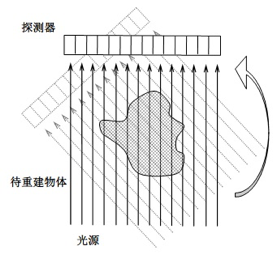
\includegraphics[width=5cm]{CT-system.png} \\
\caption{CT系统示意图} \label{chongshu1}
\end{minipage}
\hspace{1ex}
\begin{minipage}[t]{0.5\textwidth}  
\centering  
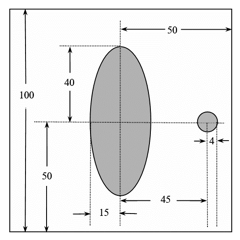
\includegraphics[width=5cm]{model-template.png}\\
\caption{模版示意图(单位:mm)}  \label{chongshu2}
\end{minipage}  
\end{figure} 

\begin{enumerate}
	\item 在如图(\ref{chongshu2})所示的正方形托盘上放置两个均匀固体介质组成的标定模板,根据这一模板及其接收信息,确定CT系统旋转中心在正方形托盘中的位置、探测器单元之间的距离以及该CT系统使用的X射线的180个方向。
	\item 利用上述CT系统得到某未知介质的接收信息。在(1)的标定基础上,确定该未知介质在正方形托盘中的位置、几何形状和吸收率等信息。具体给出题中给出的10个位置处的吸收率。
	\item 利用上述CT系统得到另一个未知介质的接收信息。在(1)的标定基础上,给出该未知介质的相关信息。同(2)给出10个位置出的吸收率。
	\item 分析(1)中参数标定的精度和稳定性。在此基础上自行设计新模板、建立对应的标定模型,以改进标定精度和稳定性,并说明理由。
\end{enumerate}

\section{问题分析}
\par CT系统在安装过程中往往会存在机械误差,而这些误差对物体重建的准确性影响是至关重要的,本文对如何确定标定系统的参数、通过接收信息矩阵如何还原二维图像及对新建立的模版的精度和稳定性这三个问题展开探究。 
\par 本文首先需要通过题中给定的标定模板,即正方形托盘上的两个均匀介质,通过两均匀介质的吸收率矩阵和接收信息矩阵得出CT系统旋转中心在正方形托盘中的位置,探测器单元间的距离,以及CT系统使用的X射线的180个方向。 本文发现当X射线方向为水平和竖直方向时,接收信息(吸收率延X射线方向的积分)能取得极值。因而通过比对接受信息和标定模板,结合标定模板的对称性,找到X射线方向为水平和竖直方向时对应的接受信息中的旋转次数,再结合几何位置、小圆半径的对应关系依次确定旋转中心以及探测器单元间距d。本文发现X射线方向为水平方向和竖直方向时,可以找出对应的旋转次数,并可以求出每次的旋转平均角度,本文先假设每次采用该平均旋转角度均匀扫描,后用该平均旋转角度去还原图像并进行检验。
\par 之后本文需要通过附件三某未知介质的接收信息矩阵确定出该未知介质在正方形托盘中的位置,以及该未知介质的几何形状和吸收率的信息,并且要求给出10个特定点的吸收率。本文先用傅里叶切片定理以及卷积反投影的方法对图像进行还原,再得到并参照附件一建立吸收率的比例系数模型,对卷积反投影得出的图像求出任意一点的相对吸收率,通过坐标可以确定10个特定点的相对吸收率的大小。
\par 接着本文需要通过附件五中的接收信息矩阵确定出该未知介质的相关信息,由于附件五中每一点都存在吸收率,本文认为该接收信息矩阵存在噪声,通过对附件五的接收信息矩阵进行卷积反投影还原,可以得出重构的图像,观察发现重构图像的轮廓不是很清晰,内部连续性不好,考虑可能存在非线性,非平稳噪声,因此采用小波滤波,对图像进行降噪处理。将降噪后的信息再进行卷积反投影重构图像,最后得出图像上各点的相对吸收率,并求出给定特定10个坐标点下的相对吸收率。
\par 最后本题要求给出新的设计模板,使得在对CT成像仪的参数确定上经度更高,稳定性更强。经度更高即是指设计出的该模板对CT系统旋转中心的确定的准确性要比原标定模板的准确性高,并且本文运用新设计的标定模板产生的旋转中心去还原原图形的重合度高于原设计的标定模板产生的旋转中心去还原原图形的重合度。稳定性更强一方面是指在加入外界噪声时,新模板标定旋转中心坐标的改变要比原模板标定的旋转中心坐标的改变小,另一方面,对系统初始参数的改变,当观察到新设计模板对图像的还原度较原设计模板高时说明新模版对图像的还原受到初始参数改变的影响较小,更加稳定。本文在考虑参数标定时仅考虑对旋转中心的标定是因为探测器单元间的距离,以及CT系统使用的X射线的180个方向直接受到旋转中心确定的影响。


\section{模型假设}
\begin{enumerate}
	\item X射线的发射器、探测器相对位置固定不变。
	\item 发射器发射的X射线能量恒定。
	\item X射线在穿过物体时不发生散射。
	\item 所有重建图像均用$256\times256$的矩阵表示。
\end{enumerate}

\section{符号说明}
\subsection{名词解释}
\begin{enumerate}
	\item \textbf{接收信息矩阵}:CT扫描系统得到的某未知介质的接收信息所构成的矩阵。
	\item \textbf{吸收率矩阵}:矩阵中每个元素反映了该点的吸收强度。
\end{enumerate}
\subsection{变量说明}
\begin{table}[!h]
\centering

\begin{tabular}{ccc}
\toprule
\makebox[0.2\textwidth][c]{符号}	&  \makebox[0.4\textwidth][c]{意义} &  \makebox[0.2\textwidth][c]{单位} \\
\midrule
$COR$ & CT旋转中心 & -\\
$f(x,y)$ & 原图像的直角坐标方程 & -\\
$F(\omega_1,\omega_2)$ & 原图像傅立叶变化后的方程 &- \\
$f(r,\theta)$ & 原图像的极坐标方程 & -\\
$J$ & 雅可比符号 & -\\
$\varphi$ & X射线与平面直角坐标系正方向的夹角 & 度($^o$)\\
$p$ & 接收信息 & -\\
$F\{\}$ & 傅立叶变换 & -\\
$F^{-1}\{\}$ & 傅立叶逆变换 & -\\
$dataTable$ & 接收信息矩阵 & -\\
$n$ & 系统旋转次数 & 次\\
$k$ & 接收器单元序号 & -\\
$d$ & 接收器单元间距 & 毫米(mm)\\
$D$ & 原标定模版小圆直径 & 毫米(mm)\\
$\alpha$ & X射线与X正半轴的夹角 & 度($^o$) \\


\bottomrule 
\end{tabular}
\end{table}


\newpage
\section{模型建立与求解}
\subsection{CT系统的参数标定}
\par 本题要求给出CT系统旋转中心在正方形托盘中的位置、探测器单元之间的距离以及该CT系统使用的X射线的180个方向。运用接收信息矩阵的局部极值,确定旋转中心的位置,并结合标定模板的对称性,找到X射线方向为水平和竖直方向时对应的接受信息中的旋转次数,再结合几何位置、小圆半径的对应关系依次确定所求参数。
\subsubsection{模型建立}

\par 以正方形托盘的左下角做为原点,下边框自左向右方向为X轴正方向,左边框自下向上方向为Y轴正方向建立平面直角坐标系,如下图(\ref{fig:q1-zuobiaoxi2})所示。在坐标系中,椭圆标定模版中心为$O_1(50,50)$,圆形标定模版圆心为$O_2(95,50)$。

\begin{figure}[!htbp]  
\begin{minipage}[t]{0.5\textwidth}
\centering  
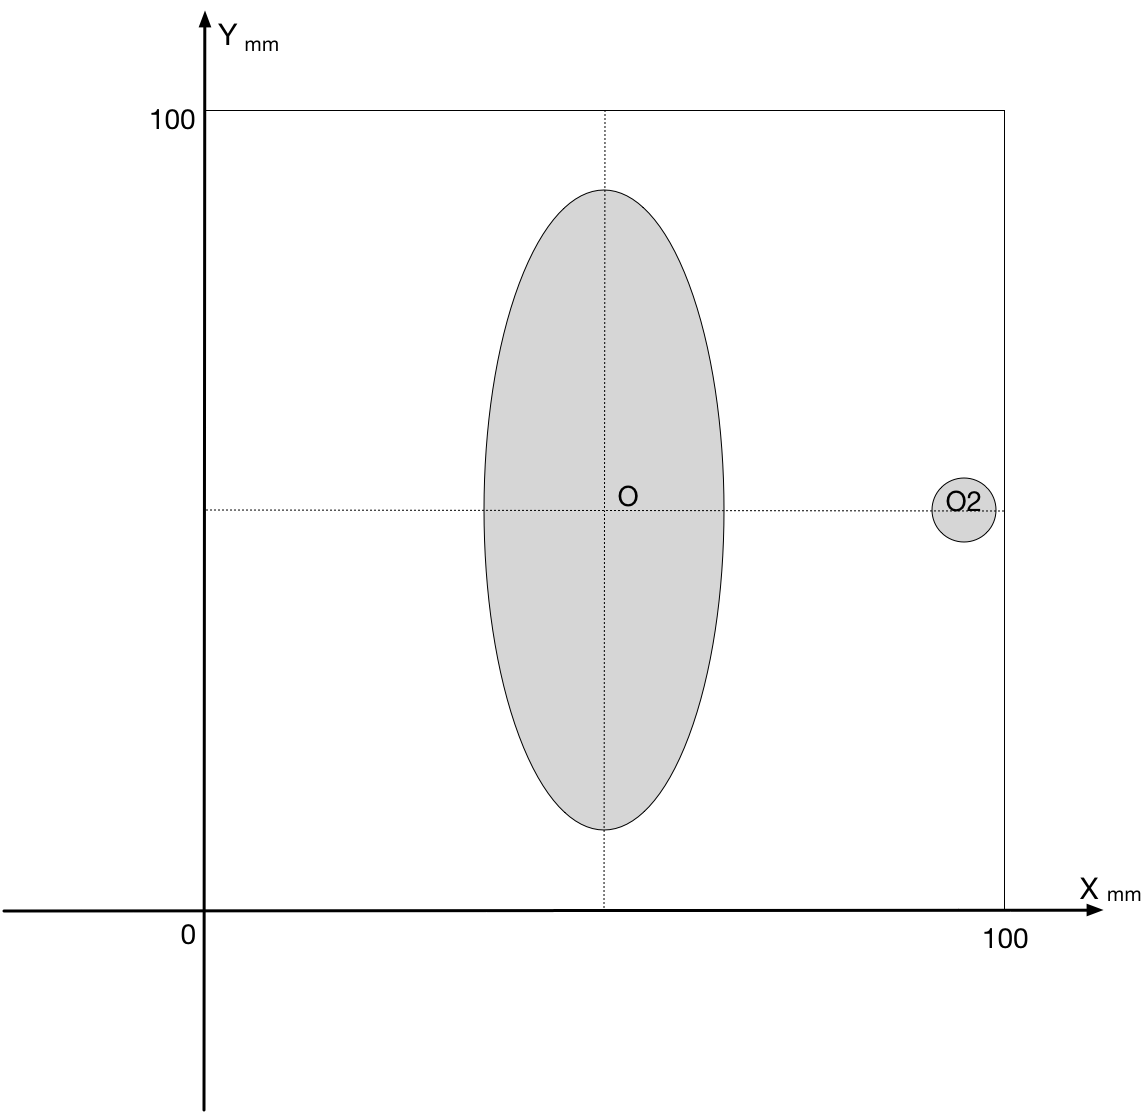
\includegraphics[width=5cm]{q1-zuobiaoxi2.png} \\
\caption{坐标系建立(单位:mm)} \label{fig:q1-zuobiaoxi2}
\end{minipage}
\hspace{1ex}
\begin{minipage}[t]{0.5\textwidth}  
\centering  
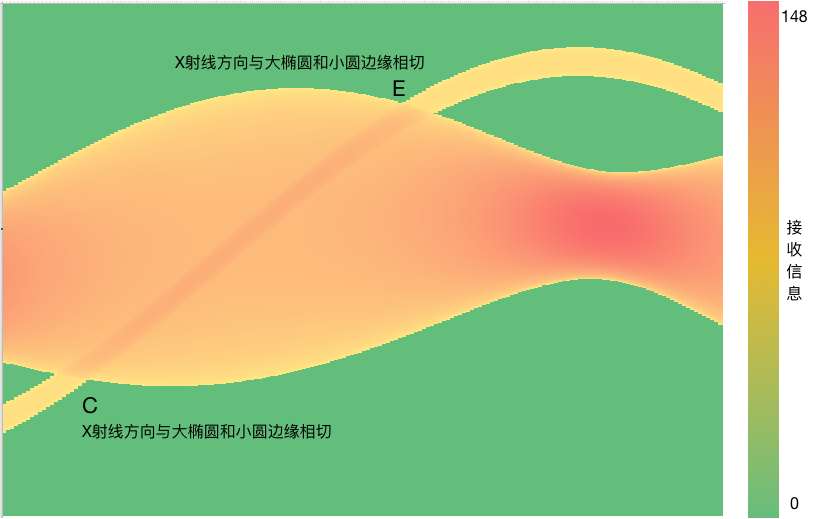
\includegraphics[width=\linewidth]{q1-table2-sejie.png}\\
\caption{附件二探测器接收信息色阶图}  \label{fig:q1-table2-sejie}
\end{minipage}  
\end{figure} 

\par 通过分析附件二的接收信息色阶图(如图(\ref{fig:q1-table2-sejie})所示),可以发现小圆的接收信息近似为一条相对窄的有宽度的正弦曲线,大椭圆的接收信息为中部的区域块。当这两个区域重叠时,即是X射线同时穿过了小圆和大椭圆。由于整个发射-接收系统是绕某固定的旋转中心进行逆时针,结合接收信息的相关数据,如通过小圆和大椭圆的相对位置等可大致判断出探测器旋转的起点和终点(如图(\ref{L1})所示)。

\par 由于模板是匀质介质,X射线穿过的介质的长度达到极值时,即当X射线方向为水平和竖直方向时,接收信息(吸收率延X射线方向的积分)能取得极值。X射线方向为竖直方向时,发射穿过大椭圆长半轴的那一条X射线的探测器会取得极值,这个极值是全局最大值,可对接收信息直接搜索得到。X射线为水平方向时,发射穿过大椭圆短半轴的那一条X射线的探测器会取得极值,但可能因为误差不明显。因而通过对称性(如图(\ref{L2})所示)来求X射线为水平方向时对应的接收信息。

\begin{figure}[!htbp]  
\begin{minipage}[t]{0.5\textwidth}
\centering  
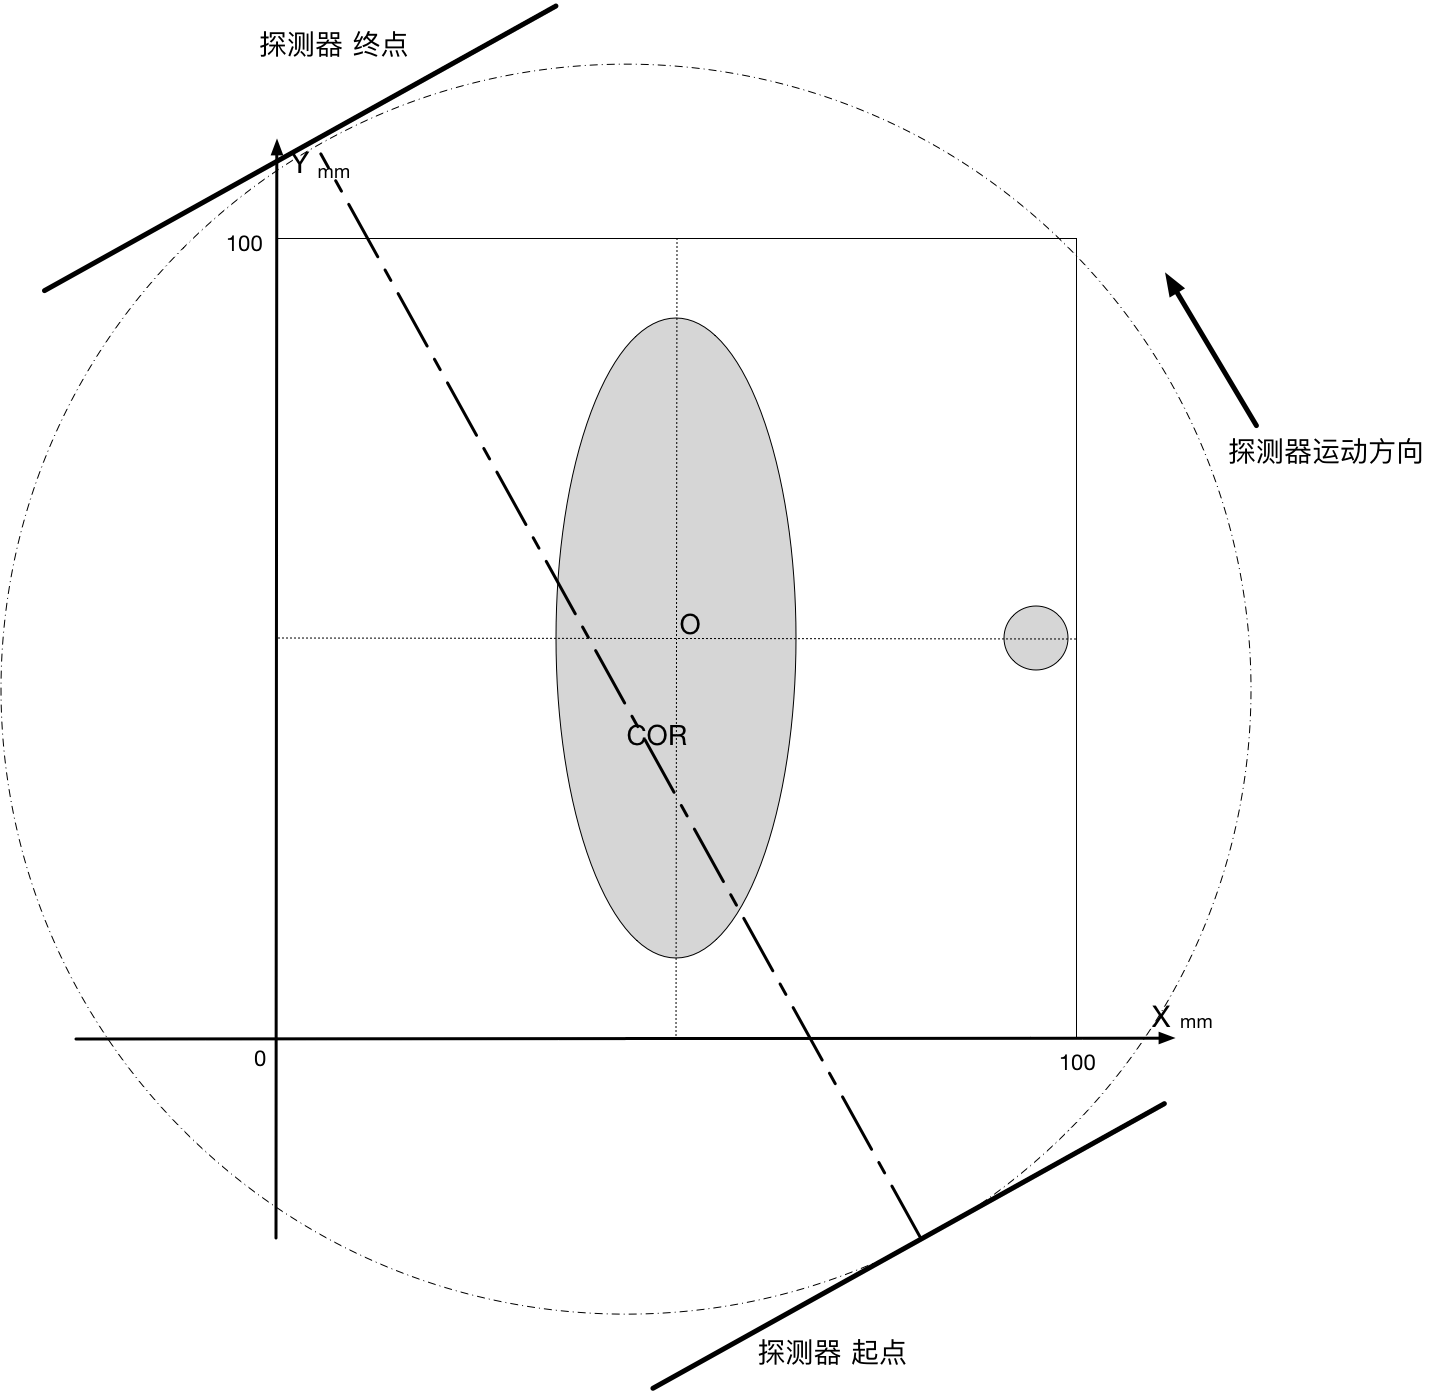
\includegraphics[width=\linewidth]{q1-3-ans.png} \\
\caption{探测器旋转路径示意图} \label{L1}
\end{minipage}
\hspace{1ex}
\begin{minipage}[t]{0.5\textwidth}  
\centering  
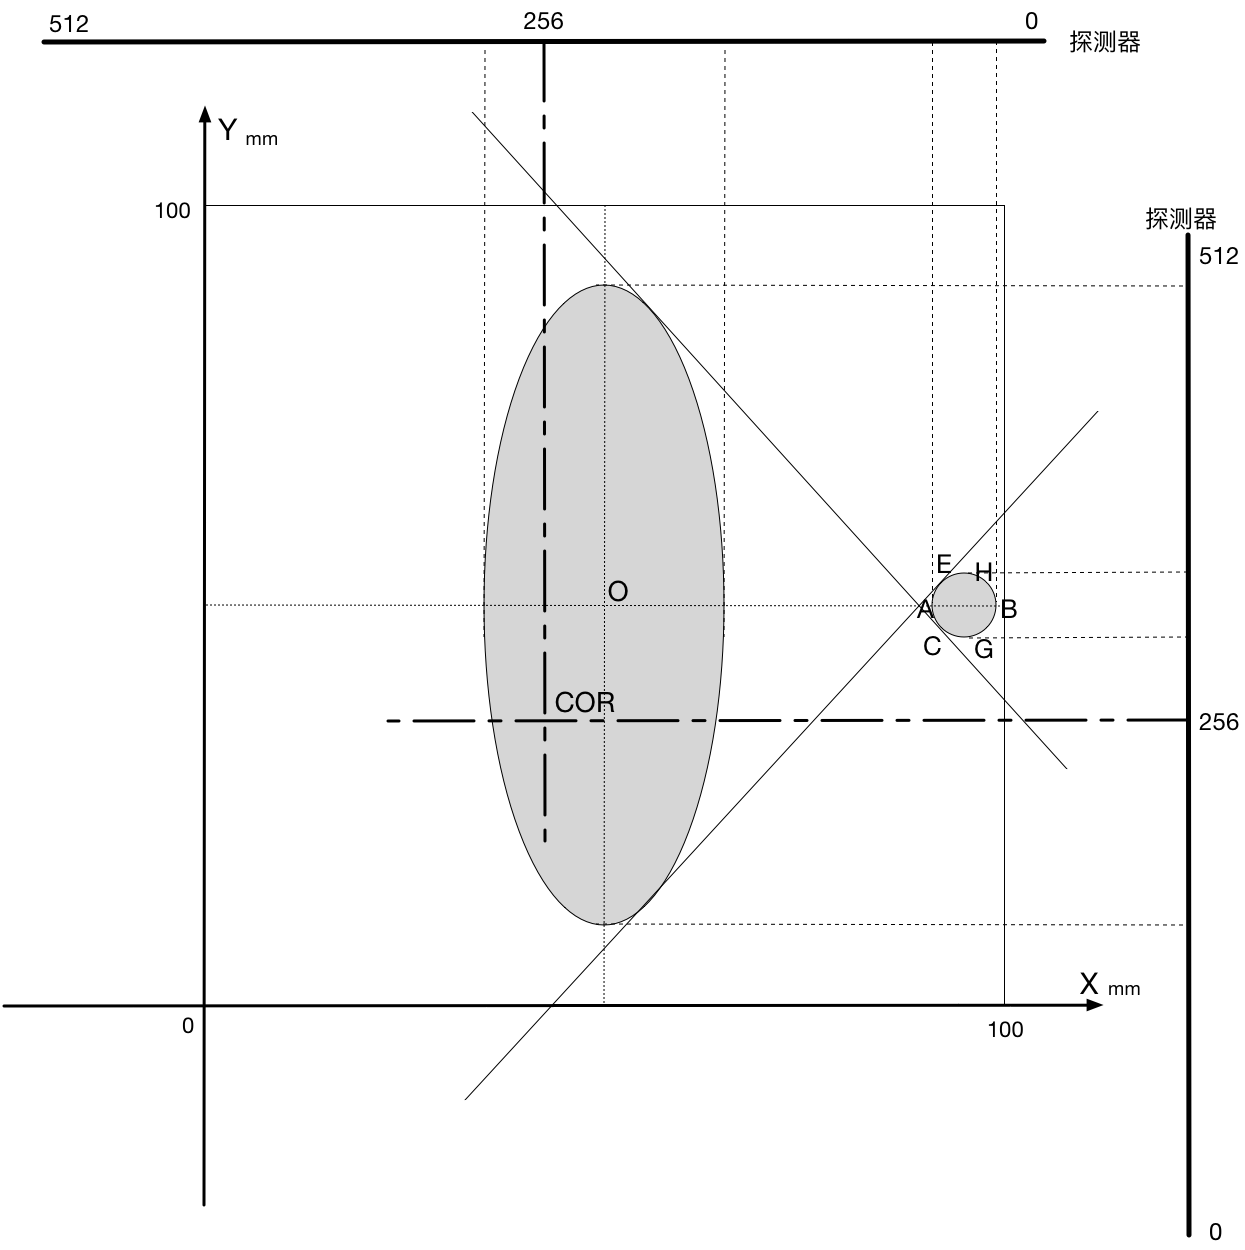
\includegraphics[width=\linewidth]{q1-zuobiaoxi-1.png}\\
\caption{旋转中心定位原理示意图}  \label{L2}
\end{minipage}  
\end{figure} 

\begin{equation}
	\label{q1-eq-1}
	\left\{
	\begin{split}
		& k = dataTable_{row}\\
		& n = dataTable_{column}\\
	\end{split}
	\right.
\end{equation}
\par 如公式(\ref{q1-eq-1})所示,接收信息矩阵$dataTable$的行数$row$是探测器的序号$k$,接受信息的列数$column$是扫描次数$n \quad (n = 1,2,\cdots,180)$。对于矩阵中的每一个点对应的探测器序号$k$和扫描次数$n$,也采取相同的表示方式。下面结合以上分析对X射线方向为垂直和水平方向具体讨论。

\textbf{a. X射线方向为竖直方向}


\begin{equation}
	\label{q1-eq-2}
	\left\{
	\begin{split}[l]
		& n_{\perp} = MAX(dataTable_{column})\\
		& D = (B_{row} - A_{row}) \cdot d_{\perp}\\ 
	\end{split}
	\right.
\end{equation}

公式(\ref{q1-eq-2})中$n_{\perp}$为X射线为垂直方向时对应的扫描次数,$A$、$B$分别为X射线水平时与小圆相切的左端点和右端点(如图(\ref{L2})所示),$D$为小圆直径,$d_{\perp}$为X射线方向为垂直方向时计算出的探测器单元间距。

\textbf{b. X射线方向为水平方向}

\begin{equation}
	\label{q1-eq-3}
	\left\{
	\begin{split}
	& n_{\parallel} = \frac{1}{2}(E_{column} + C_{column})\\
	& D = (H_{row} - G_{row}) \cdot d_{\parallel}\\ 	
	\end{split}
	\right.
\end{equation}

公式(\ref{q1-eq-3})中$n_{\parallel}$为X射线为水平方向时对应的扫描次数,$C$、$E$分别为X射线与大椭圆和小圆边缘同时相切与小圆的两个切点,$H$、$G$分别为X射线竖直时与小圆相切的上端点和下端点(如图(\ref{L2})所示),$D$为小圆直径,$d_{\parallel}$为X射线方向为垂直方向时计算出的探测器单元间距。

综合以上公式\ref{q1-eq-1}、\ref{q1-eq-2},可以得到旋转中心COR和探测器单元间距的表达式。


\paragraph*{(1)旋转中心$COR$位置确定}~\\

\par 旋转中心即为X射线方向为水平和竖直方向时,所对应探测器中垂线的交点。
\begin{equation}
	\label{q1-eq-4}
	\left\{
	\begin{split}
		COR_{row} = \frac{512}{2} = 256 \\
		COR_{x} = O_{x} - (O_{row} - COR_{row}) \cdot d \\
		COR_{y} = O_{y} - (O_{row} - COR_{row}) \cdot d \\
	\end{split}
	\right.
\end{equation}
公式(\ref{q1-eq-4})中$COR$是旋转中心,$O$是大椭圆的中心,$d$是探测器单元间距。

\paragraph*{(2)探测器单元间距$d$确定}~\\

探测器单元间距为$d_{\parallel}$和$d_{\perp}$的平均值。代入公式(\ref{q1-eq-2}、\ref{q1-eq-3})得到以下计算公式(\ref{q1-eq-5})
\begin{equation}
	\label{q1-eq-5}
	d = \frac{1}{2}(d_{\perp} + d_{\parallel}) = \frac{1}{2} \left( \frac{D}{B_{row} - A_{row}} + \frac{D}{H_{row} - G_{row}} \right)
\end{equation}

公式(\ref{q1-eq-5})中$d_{\parallel}$和$d_{\perp}$分别为X射线方向为垂直、水平方向时计算出的探测器单元间距,$A$、$B$分别为X射线水平时与小圆相切的左端点和右端点,$D$为小圆直径,$H$、$G$分别为X射线竖直时与小圆相切的上端点和下端点。

\paragraph*{(3)CT系统使用的180个方向的确定}~\\

通过分析,发现$n_{\perp}$与$n_{\parallel}$之差恰好为$90$,即X射线方向从水平方向转到竖直方向刚好旋转了90次,猜想是一度一次均匀转动,因而X射线初始方向与X轴正方向的夹角$\alpha_1$和X射线转到水平方向的旋转次数$n_{\parallel}$在数值上相等,并在模型求解中给出了具体验证。

\begin{equation}
	\label{q1-eq-6}
	\left\{
	\begin{split}
		& \alpha_1 = n_{\parallel} = \frac{1}{2}(E_{column} + C_{column})\\
		& \alpha_i = \mid \alpha_1 -  (i-1) \mid \quad (i = 1,2,\cdots,180)\\
	\end{split}
	\right.
\end{equation}

公式(\ref{q1-eq-6})中,$\alpha_1$为X射线初始方向与x轴正方向的夹角,一次$1^o$转动,从第四象限转到第二象限,$\alpha_1,\alpha_2,\cdots,\alpha_{180}$分别表示CT系统使用的180个方向。

\subsubsection{模型求解}
根据模型,给出求解算法如下所示:
\begin{enumerate}
	\item 将原图像的点$A$、$B$、$C$、$E$、$O$、$G$、$H$分别与附近二中$512\times 180$的接收信息矩阵按欧式距离最小的规则对应。
	\item 通过对接收信息矩阵$dataTable$遍历得到最大值得到$n_{\perp}$。
	\item 通过对称性结合公式(\ref{q1-eq-3})得到$n_{\parallel}$。
	\item 通过公式(\ref{q1-eq-5})求得探测器单元间距$d$。
	\item 通过公式(\ref{q1-eq-4})求得旋转中心$COR$位置。
	\item 通过(\ref{q1-eq-6})求得CT系统使用的$180$个角度。
\end{enumerate}
\paragraph*{(1)旋转中心$COR$位置确定}~\\

\par 经过求解,旋转中心$COR$在托盘中的位置为:距托盘左边缘$40.8966mm$,据托盘下侧边缘$55.7931mm$($COR$位置如图(\ref{fig:q1-3-ans2})所示)。

\paragraph*{(2)探测器单元间距$d$确定}~\\
\par 经过求解,$d = 0.2759mm$
\paragraph*{(3)CT系统使用的180个方向的确定}~\\

\par 经过求解,当X射线方向为水平方向时,旋转次数$n_{\parallel}=61$。当X射线方向为竖直方向时,旋转次数$n_{\perp}=151$。发现$n_{\perp}$与$n_{\parallel}$之差恰好为$90$,先假设装置是每次$1^o$均匀转动,再分等间距扫描方式($0.97^o$和$1.03^o$)和非等间距扫描方式($0.5^o$、$1.5^o$交替进行)进行模型检验,分别重建图像(具体重建模型在下一小节:基于卷积反投影的CT图像重建中给出),并与等间距扫描方式($1^o$)重建的图像及原始图像进行比较(如图\ref{q1-180} $\sim$ \ref{q1-185}所示)。
\begin{figure}[!htbp]  
\begin{minipage}[t]{0.5\textwidth}
\centering  
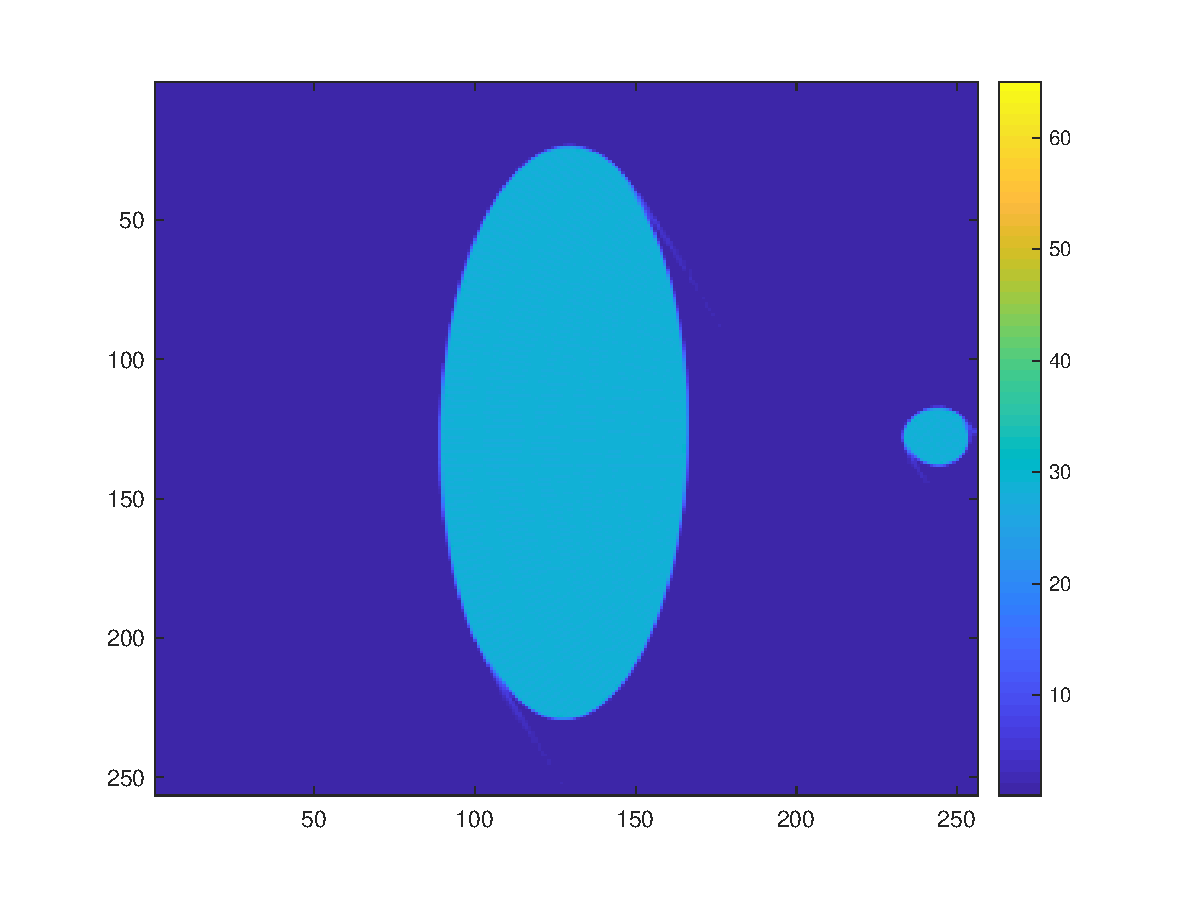
\includegraphics[width=\linewidth]{q1-180.eps} \\
\caption{均匀间距$1^o$时重建结果} \label{q1-180}
\end{minipage}
\hspace{1ex}
\begin{minipage}[t]{0.5\textwidth}  
\centering  
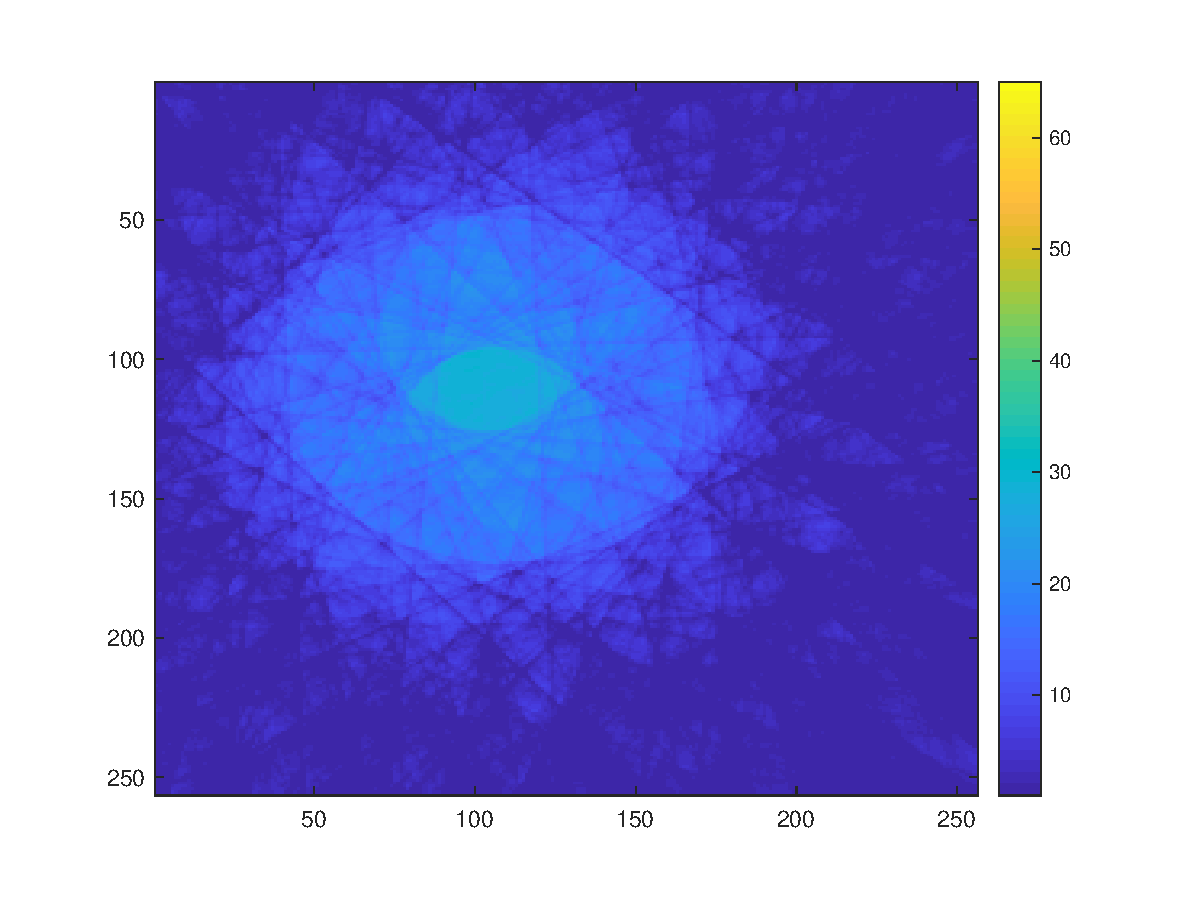
\includegraphics[width=\linewidth]{q1-05.eps}\\
\caption{非均匀间距$0.5^o$|$1.5^o$交替时重建结果}  \label{q1-05}
\end{minipage}  
\end{figure} 

\begin{figure}[!htbp]  
\begin{minipage}[t]{0.5\textwidth}
\centering  
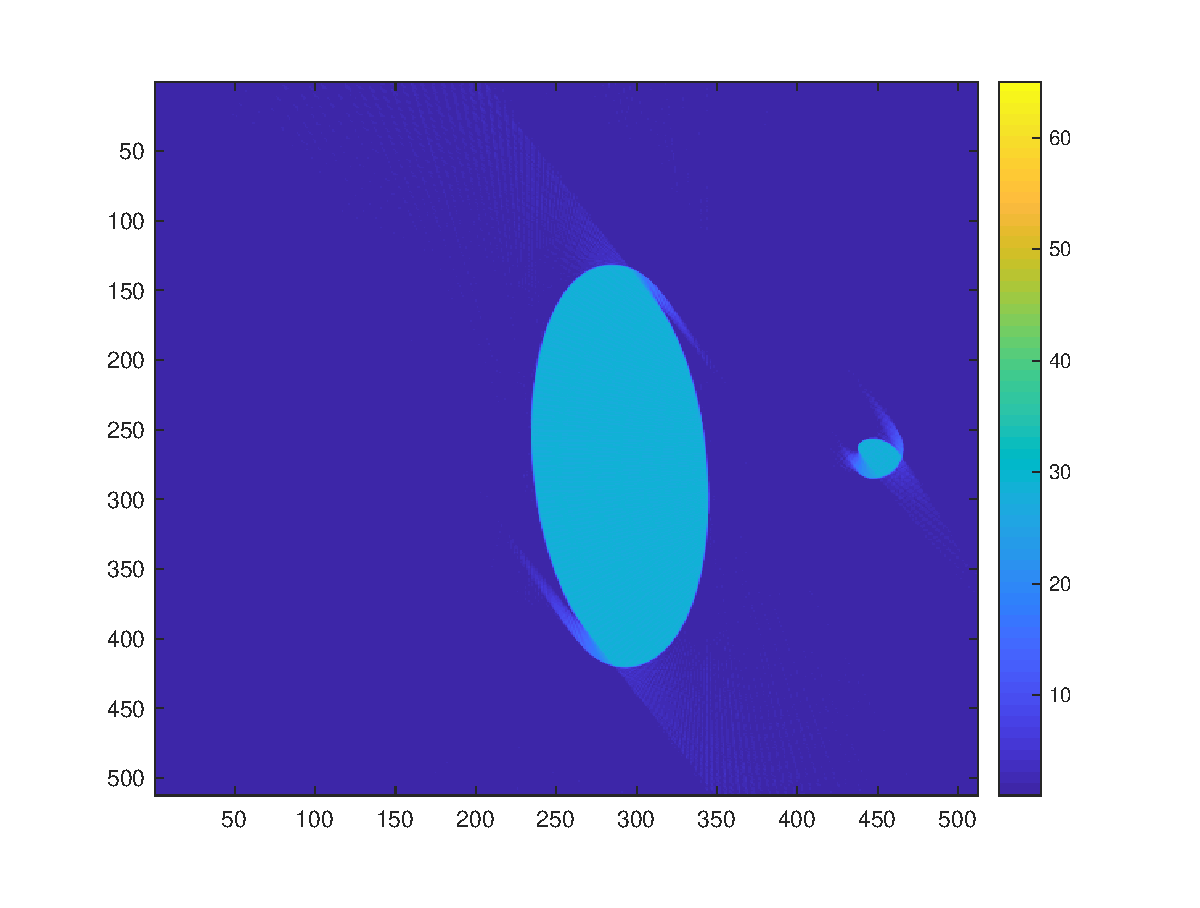
\includegraphics[width=\linewidth]{q1-175.eps} \\
\caption{均匀间距$(1.03^o$时重建结果} \label{q1-175}
\end{minipage}
\hspace{1ex}
\begin{minipage}[t]{0.5\textwidth}  
\centering  
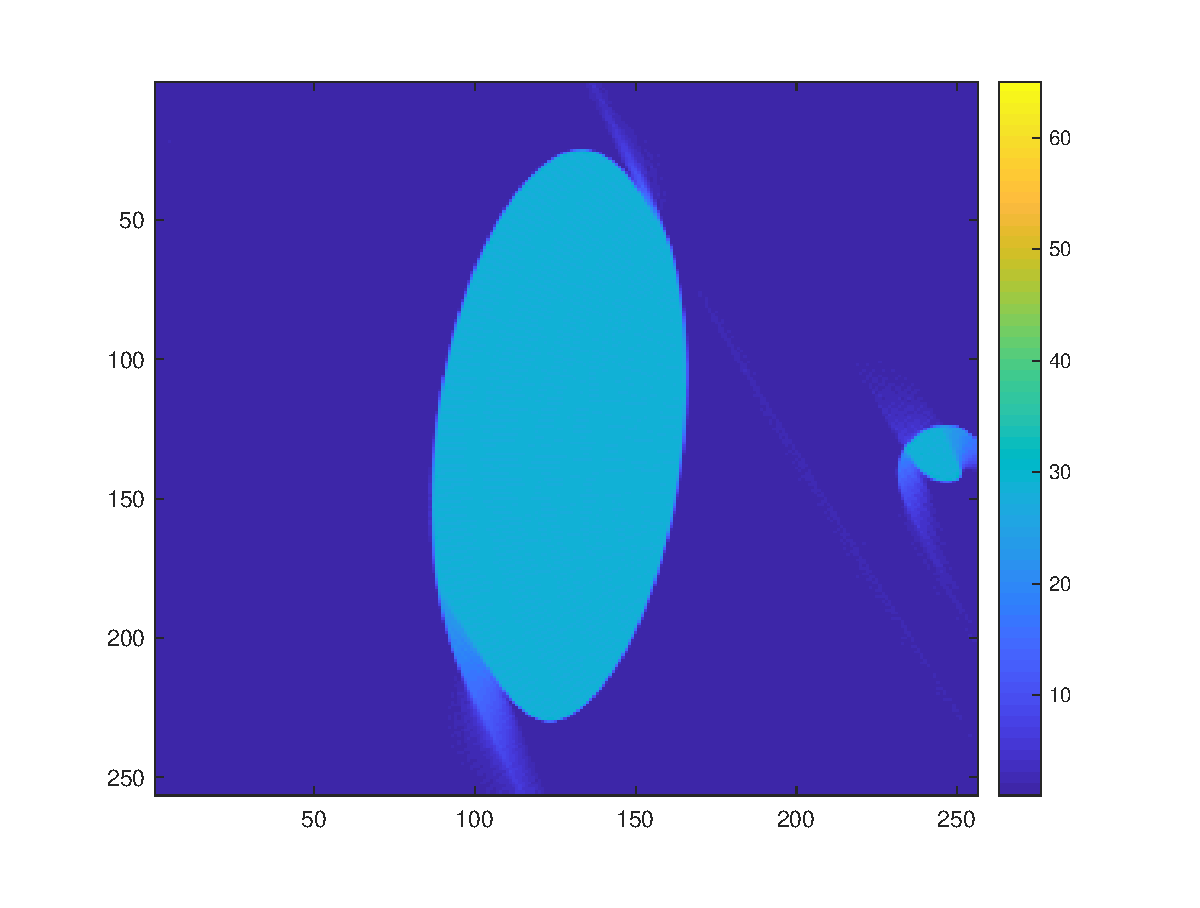
\includegraphics[width=\linewidth]{q1-185.eps}\\
\caption{均匀间距$(0.97^o$时重建结果}  \label{q1-185}
\end{minipage}  
\end{figure} 

等间距扫描($1^o$)方式重建的图像如图(\ref{q1-180})所示,观察发现等间距扫描方式重建的图像与原图像非常相近,还原效果好。


非等间距扫描($0.5^o$、$1.5^o$交替进行)方式重建的图像如图(\ref{q1-05}),观察发现重建的图像重影严重,图像已经无法识别。

等间距扫描($0.97^o$、$1.03^o$)方式重建的图像如图\ref{q1-175}、\ref{q1-185},观察发现即便仅有$0.03^o$的偏差,重建的图像轮廓已开始出现毛刺和畸变。

因而可以认为我们的假设是正确,再通过公式(\ref{q1-eq-6})求得X射线初始方向与X正半轴顺时针夹角为$61^o$,经过180次$1^o$的逆时针旋转,最终与X正半轴夹角$119^o$(如图(\ref{fig:q1-3-ans})所示)。
\begin{figure}[!htbp]  
\begin{minipage}[t]{0.5\textwidth}
\centering  
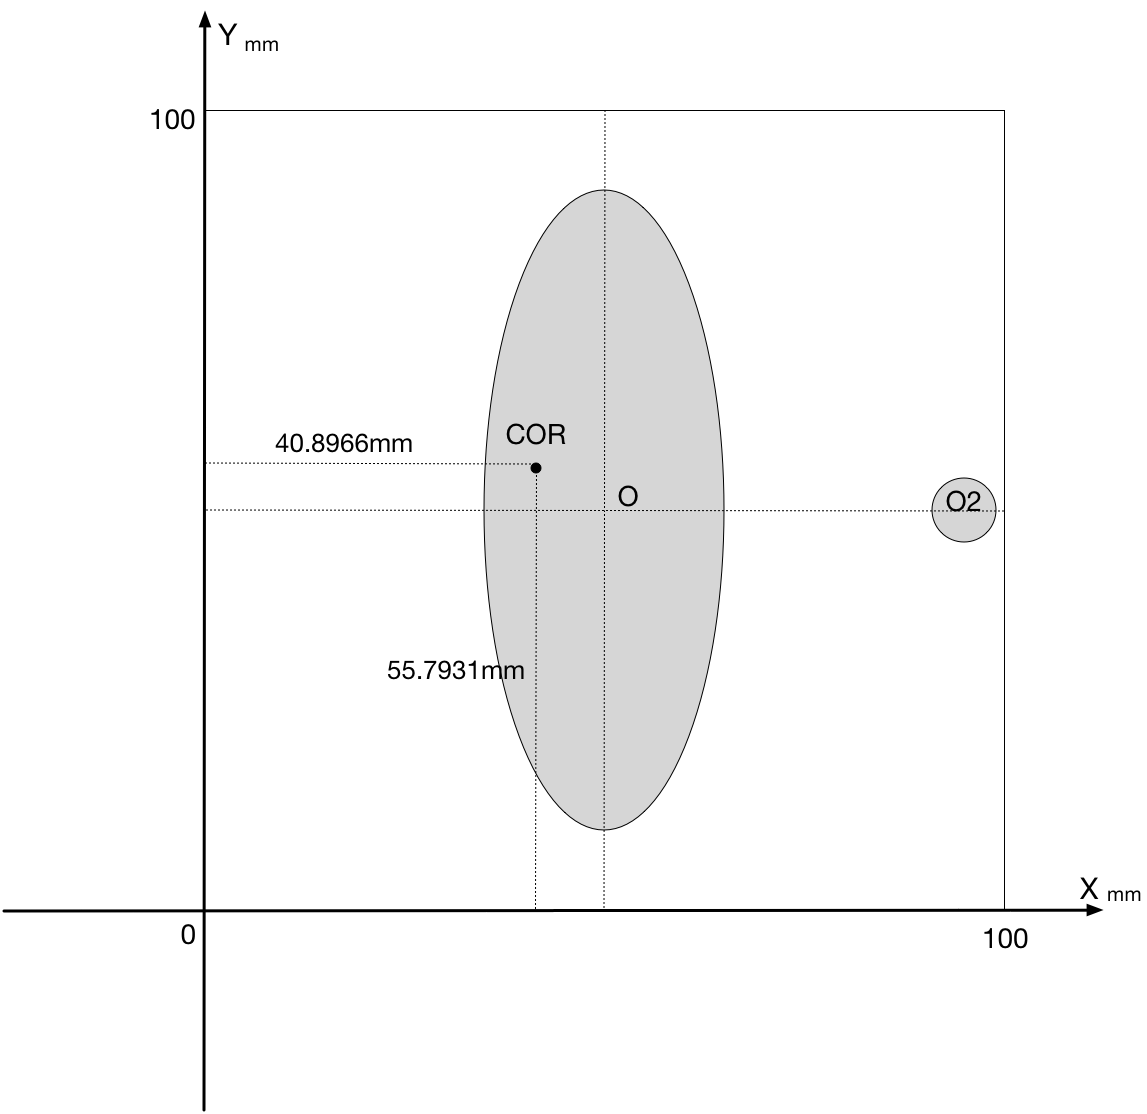
\includegraphics[width=5.5cm]{q1-3-ans-2.png} \\
\caption{旋转中心$COR$位置示意图} \label{fig:q1-3-ans2}
\end{minipage}
\hspace{1ex}
\begin{minipage}[t]{0.5\textwidth}  
\centering  
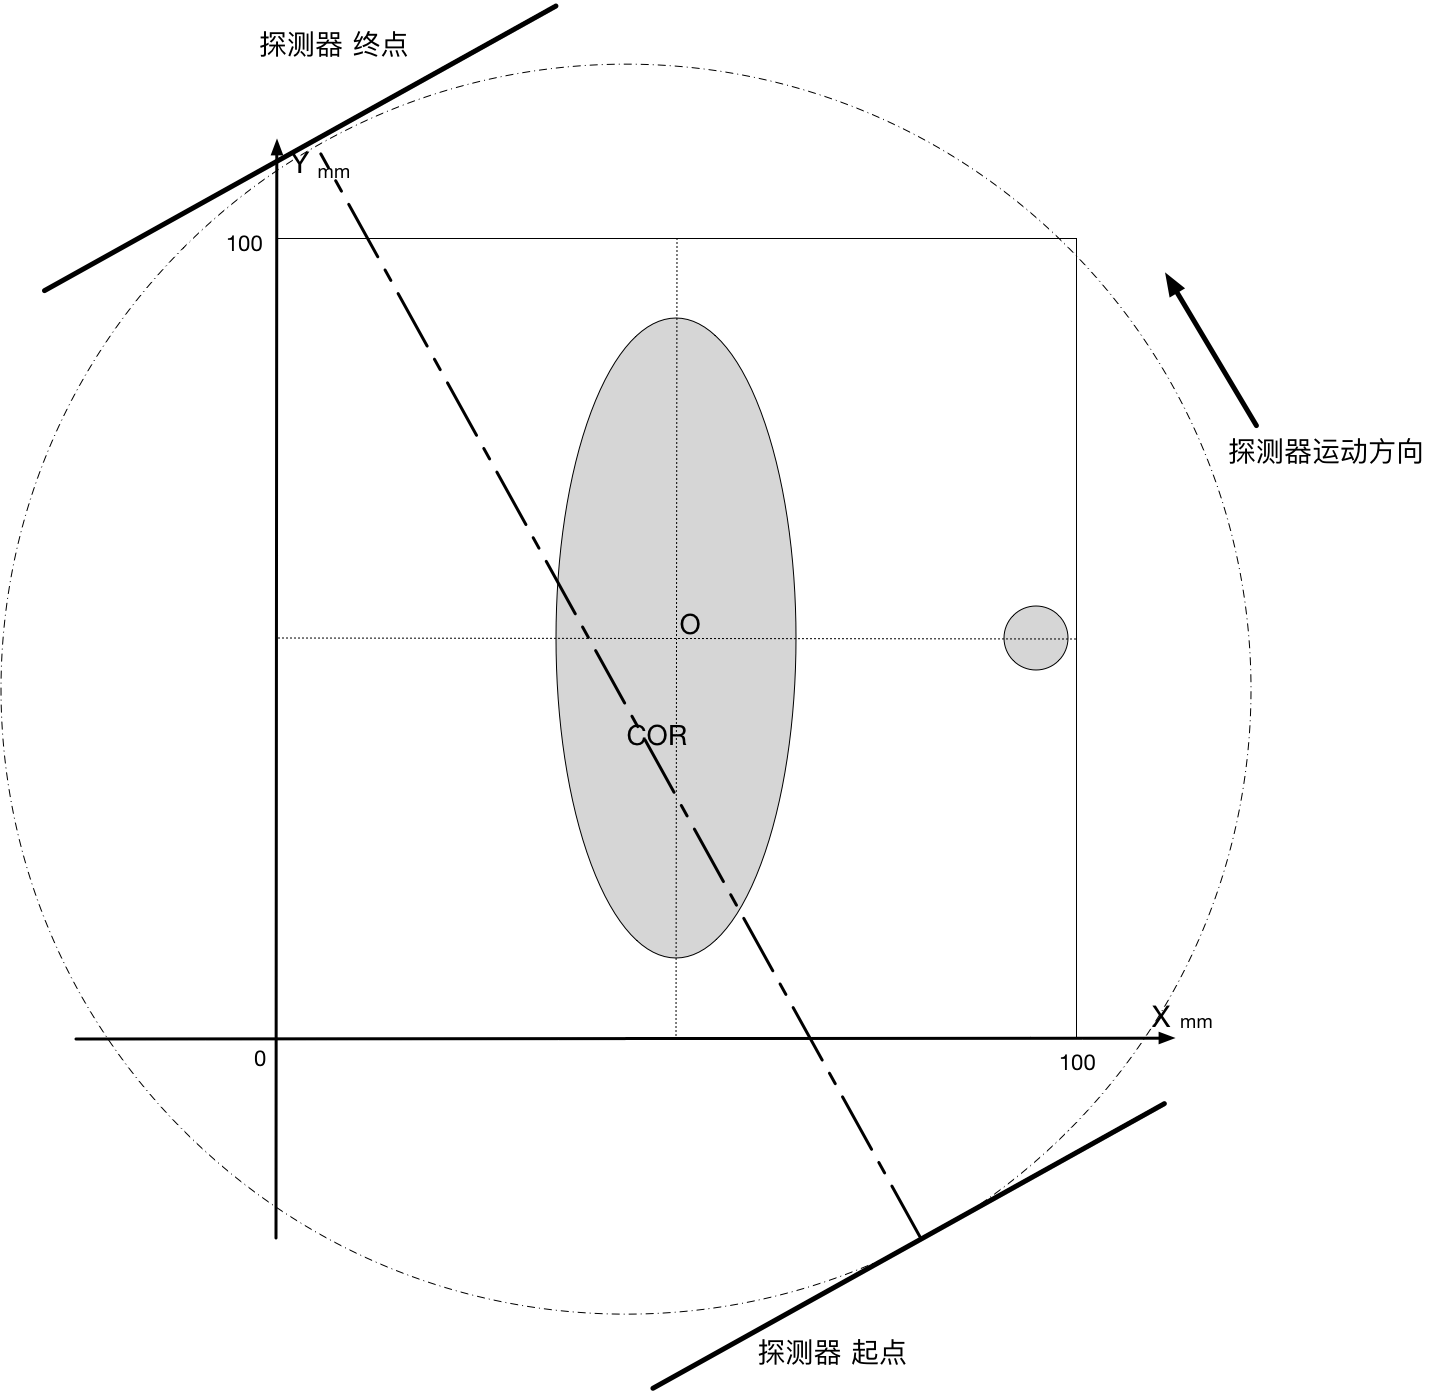
\includegraphics[width=5.5cm]{q1-3-ans.png}\\
\caption{探测器旋转路径示意图}  \label{fig:q1-3-ans}
\end{minipage}  
\end{figure} 

\newpage
\subsection{基于卷积反投影的CT图像重建}
\subsubsection{模型建立}
\paragraph*{(1)卷积反投影法图像重建}~\\
\par 利用卷积反投影法重建图像时,先把由检测器上获得的原始数据与一个滤波函数进行了卷积运算,得到各方向卷积的投影函数;然后再把它们从各方向进行反投影,即按其原路径平均分配到每一矩阵元上,进行叠加后得到每一矩阵元的CT值;再经过适当处理后就可以得到被扫描物体的断层图像。

\par 设原图像的二维表达式为$f(x,y)$,其定义如下公式(\ref{m1-1})所示。
\begin{equation}
\label{m1-1}
	f(x,y) = F^{-1} [F(\omega_1, \omega_2)]
\end{equation}
其中$F(\omega_1,\omega_2)$为$f(x,y)$的二维傅立叶变换\upcite{fuliye}
(如公式(\ref{m1-2})所示)。
\begin{equation}
	\label{m1-2}
	F(\omega_1,\omega_2) = \int^{+\infty}_{-\infty}\int^{+\infty}_{-\infty} f(x,y) e^{-j2\pi(\omega_1 x + \omega_2 y)} dxdy
\end{equation}
由二维傅立叶变换逆变换可得公式(\ref{m1-3}),
\begin{equation}
	\label{m1-3}
	f(x,y) =\frac{1}{4\pi^2} \int^{+\infty}_{-\infty}\int^{+\infty}_{-\infty} F(\omega_1,\omega_2) e^{j2\pi(\omega_1 x + \omega_2 y)} d\omega_1 d\omega_2
\end{equation}
其中
\begin{equation}
	\label{m1-4}
	\omega_1 x + \omega_2 y = \rho (xcos\varphi +ysin\varphi)
\end{equation}
可理解为在频域进行坐标变换(如公式(\ref{m1-5})所示)。


\begin{equation}
	\label{m1-5}
	\left\{
	\begin{split}
		& \omega_1 = \rho cos\varphi \\
		& \omega_2 = \rho sin\varphi \\
	\end{split}
	\right.
\end{equation}


\begin{figure}[h]
\small
\centering
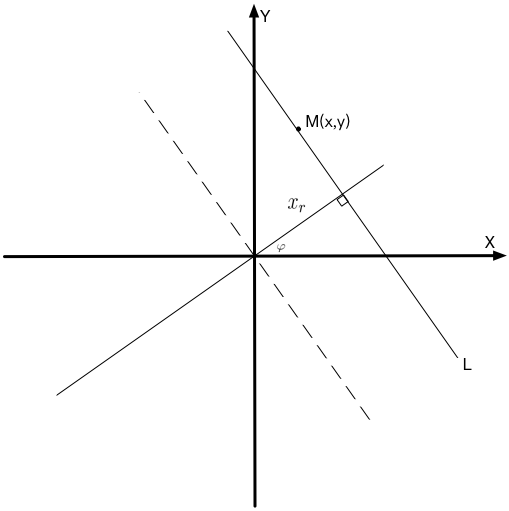
\includegraphics[width=8cm]{m1-1.png}
\caption{坐标关系示意图} \label{fig:m1-1}
\end{figure}


如图(\ref{fig:m1-1})所示,对于线$L$上的点, 为坐标原点到线$L$的距离,表示线$L$法线方向与直角坐标系X轴正方向的夹角。因此$x_r = y sin\varphi + x cos \varphi$,其中$M(x,y)$为X射线通过图像中的一点,在极坐标系中$M$的坐标也可以表示为$(r,\theta)$。其中$r$为$M$与坐标原点$O$的距离,$\theta$为$OM$与极轴的夹角。因此,公式(\ref{m1-4})可化为如下公式(\ref{m1-6})所示的形式。 
\begin{equation}
	\label{m1-6}
	\omega_1 x + \omega_2 y = 2\pi \rho (x cos\varphi + y sin\varphi) = 2\pi \rho x_r = 2\pi\rho r cos (\theta - \varphi)
\end{equation}

将公式(\ref{m1-3})进行坐标变换,其中$d \omega_1 d \omega_2  = \mid J \mid d\rho d\varphi$,雅可比行列式$\mid J \mid$计算如公式(\ref{m1-7})所示。
\begin{equation}
	\label{m1-7}
J = 
\left| {\begin{array}{*{20}c}
    \frac{\partial \omega_1}{\partial \rho} & \frac{\partial \omega_1}{\partial \varphi}\\   
     \frac{\partial \omega_2}{\partial \rho} & \frac{\partial \omega_2}{\partial \varphi}\\
\end{array}} \right| = \left| {\begin{array}{*{20}c}
    2\pi cos \varphi & -2\pi \rho sin \varphi\\
    2\pi sin \varphi & 2\pi \rho cos \varphi\\   
\end{array}} \right| = 4\pi^2\rho
\end{equation}
将雅可比行列式$\mid J \mid$的计算代入$d \omega_1 d \omega_2  = \mid J \mid d\rho d\varphi$中,得到公式(\ref{m1-8}):
\begin{equation}
	\label{m1-8}
	d \omega_1 d \omega_2  = \mid J \mid d\rho d\varphi = 4\pi\rho^2 \cdot d\rho d \varphi
\end{equation}
将公式(\ref{m1-6}、\ref{m1-8})代入公式(\ref{m1-2})中,可得如下公式(\ref{m1-9})。
\begin{equation}
	\label{m1-9}
	\int^{\pi}_{0} \int_{-\infty}^{+\infty} P(\rho,\theta)e^{j2\pi\rho r cos(\theta - \varphi)} |\rho| d \rho d \varphi
\end{equation}

公式(\ref{m1-9})中$P(\rho,\theta)$为图像	$f(x,y)$经过傅立叶变换$F(\omega_1,\omega_2)$后在某一极角下的极坐标。根据傅里叶切片定理\upcite{fuliyeqiepian}
,$P(\rho,\theta)$也是$f(x,y)$在某一方向投影函数的二维傅立叶变换。
将公式(\ref{m1-9})转换为二次积分,得到公式(\ref{m1-10})如下所示。

\begin{equation}
	\label{m1-10}
	\int_{0}^{\pi} d \varphi \int_{-\infty}^{+\infty} |\rho| P(\rho,\theta)e^{j2\pi\rho r cos (\theta - \varphi)} d\rho
\end{equation}
公式(\ref{m1-10})中第一次积分过程如下公式(\ref{m1-11})所示。
\begin{equation}
	\label{m1-11}
	\int_{-\infty}^{+\infty} |\rho| P(\rho,\theta)e^{j2\pi \rho r cos (\theta-\varphi)} d \rho = h(x_r)\otimes p(x_r,\varphi) = g(x_r,\varphi)
\end{equation}

公式(\ref{m1-11})的物理意义为,投影$p(x_r,\theta)$经过$|\rho| = F[h(x_r)]$滤波器后修正的投影$g(x_r,\varphi)$在满足$x_r = r cos (\theta-\varphi)$时的值。将公式(\ref{m1-11})代入公式(\ref{m1-10})中得:
\begin{equation}
	\label{m1-12}
	\int_{0}^{\pi}g(x_r,\varphi)d\varphi = \int_{0}^{\pi} g[r cos (\theta-\varphi),\varphi]d\varphi = f(x,y)
\end{equation}
公式(\ref{m1-12})的物理意义可理解为经过给定$(r,\theta)$所有滤波后的投影在$\varphi = 0 \sim \pi$范围内的累加-反投影重建得 $(r,\theta)$点所在的吸收率叠加值。
将$f(x,y)$离散化得
\begin{equation}
	\label{m1-13}
	f(x,y) = \Delta\varphi \sum\limits_{n=0}^{N-1} g[(x cos n \Delta\varphi + y sin n \Delta\varphi),n\Delta\varphi]
\end{equation}
即
\begin{equation}
\label{m1-14}
	f(i\Delta\varphi,j\Delta\varphi) = \Delta\varphi \sum\limits_{n=0}^{N-1} g[(i\Delta x cos n \Delta\varphi + j \Delta y sin n \Delta\varphi),n\Delta\varphi]
\end{equation}
公式\ref{m1-13}和\ref{m1-14}中$\Delta\varphi$为托盘每次旋转的角度,N为总旋转次数。

\paragraph*{(2)吸收率比例系数的构建}~\\
\par 题中给出,具有512个等距单元的探测器测量待检测介质吸收衰减后的射线能量,并通过增益处理得出180组接收信息。因为对接收器的接收信息进行了处理,可以得出,附件二的吸收率经处理后,得出附件一中该均匀介质的吸收率为1,方形托盘上没有放置介质的部分的单位吸收率为0。对于第二问中某未知介质在图中特定位置的“相对吸收率”的确定,本文提出“吸收率比例系数”这一个概念,并认为 “吸收率的比例系数”是系统参数,不随检测介质不同而发生改变。

定义\textbf{吸收率比例系数$\eta$}如下公式(\ref{m2-1})所示,式中分子$I$表示吸收率,分母$I_0$表示相对吸收率。
\begin{equation}
	\label{m2-1}
	\eta = \frac{I}{I_0}
\end{equation}  

\par 本文通过附件二接收信息矩阵,通过上述“卷积反投影图像重建模型”对附件一中的图像进行重构,X射线扫描的旋转中心、初始位置、旋转次数以及每次旋转的角度均与第一问得出的系统标定参数相同。得出重构后的图像每一个像素所对应的吸收率$I$。由于原图像中仅有均匀介质和没有放置介质两部分。本文首先对得出的重构图像上各点的吸收率进行阈值分割,通过图像将吸收率小的像素点置0,即将该部分视为没有摆放介质的部分,然后本文将对剩余吸收率集中的大多数吸收率取均值,视为该均匀介质的吸收率$I$。对剩余非常少的值本文认为是合理误差,不进行考虑。

通过上式(\ref{m2-1})可以求出该系统吸收率的比例系数$\eta$。

\paragraph*{(3)模型汇总}~\\

\par 结合基于卷积反投影的CT图像重建小节中前述两个模型,本文首先对附件三的接收信息矩阵运用“滤波反投影图像重建模型”对图像进行重构,X射线扫描的旋转中心、初始位置、旋转次数以及每次旋转的角度均与第一问得出的系统标定参数相同,得出重构后的图像及重构图像中每一个像素点的吸收率I,然后运用模型二求出的$\eta$值,通过如下公式(\ref{m2-2}),求出图像中每一点的相对吸收率。
\begin{equation}
	\label{m2-2}
	I_0 = \frac{I}{\eta}
\end{equation}


\subsubsection{模型求解}

\par 附件3中给出了利用上述CT系统得到的某未知介质的接收信息。本文需要利用第一问中得到的标定参数,确定该未知介质在正方形托盘中的位置、几何形状和吸收率等信息。另外,需要给出附件4中所给的10个位置处的吸收率。模型建立中,本文已经给出了基于傅立叶中心切片定理通过接受信息还原未知介质二维图像的方法。其中,本文采用的卷积反投影法既还原了原始图像,又有效地滤除了噪声。
\par 求解算法如下:
\begin{enumerate}
	\item 读取附件3接收信息的数据,存入矩阵$dataTable(512\times180)$中。
	\item 构造数字滤波器,存入矩阵$hl(1\times 512)$中。
	\item 角度从初始角度(方向为x轴正方向逆时针旋转$61^o$)开始,逐次增加,步长为$1^o$,即循环变量$m$初始值为$1$,逐次增加,步长为$1$,将$dataTable$的第$m$列和$hl$卷积。
	\item 对(3)中确定角度,计算反投影的二维图像,即循环变量$i$、$j$初始值为1,逐次增加,步长为1,将卷积后的结果代入反投影离散求和公式,每次循环进行累加。
	\item (3)、(4)三层循环后计算出$180$次扫描对应二维图像的180次累加,得到还原的二维图像。
	\item 利用(1)中标定将图像进行缩放平移,得到$256\times 256$的原图像。
	\item 对原图像进行阈值处理,将背景置为0,并参照附件三将吸收率归一化为相对吸收率。
	\item 从图像中得到该未知介质在正方形托盘中的位置、几何形状以及附件4中所给的10个位置处的吸收率。
\end{enumerate}


\par 通过求解,得到重建的未知介质的图像如图(\ref{fig:q2-1})所示:
\begin{figure}[h]
\small
\centering
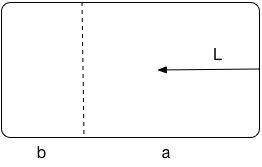
\includegraphics[width=9cm]{q2-1.png}
\caption{附件三重建的图像} \label{fig:q2-1}
\end{figure}


\par 此时得到$256\times 256$对应像素点的值还需要除以吸收率比例系数进行归一化成为相对吸收率。吸收率比例系数通过附件一进行计算。

\paragraph*{(1)吸收率比例系数,附件三相对吸收率的求解}~\\

\par 首先对附件二重建的图像的吸收率进行分析,先以1为步长,得出每个吸收率范围中的像素点个数和累计的像素点个数如表(\ref{不同吸收率范围对应的像素点个数})所示,

\begin{table}[!h]
\centering
\caption{不同吸收率范围对应的像素点个数}
\label{不同吸收率范围对应的像素点个数}
\begin{tabular}{ccc}
\toprule
吸收率范围&像素点个数&像素点累计个数\\
\midrule
<1&49706&49706\\
<2&2378&52084\\
<3&191&52275\\
<4&110&52385\\
<5&81&52466\\
$\cdots$ & $\cdots$ & $\cdots$ \\
<26&48&53079\\
<27&47&53126\\
<28&3201&56327\\
<29&9185&65512\\
<30&24&65536\\
\bottomrule 
\end{tabular}
\end{table}

\par 可见吸收率集中在$I<4$和$I>27$两个范围内。其他范围内较为稳定,可认为是受到噪声干扰的介质的过渡部分。吸收率$I<4$对应的像素点阵是受噪声干扰的无介质区域,吸收率$I>27$对应的像素点阵是标定模板的匀质区域。通过附件二可知该匀质介质吸收率为1。

\par 因而将吸收率$I>27$对应的均值作为吸收率比例系数$\eta$。计算得 $\eta=28.1145$,类似附件二重建图像的做法,首先对附件三重建图像的吸收率进行分析,为阈值处理做准备(不同吸收率范围对应的像素点个数表见附件)。

\par 可得吸收率集中在$I<4$和$I>25$两个范围内。其他范围内较为稳定,可认为是受到噪声干扰的介质的过渡部分。吸收率$I<4$对应的像素点阵是受噪声干扰的无介质区域,吸收率$I>25$对应的像素点阵是某未知介质的区域。将受噪声干扰的无介质区域对应的$I<4$的吸收率置为0,将剩余部分对应的吸收率$I$除以吸收率比例系数,得到相对吸收率,得到一个新的$256\times 256$的相对吸收率矩阵。
\par 为避免将受噪声干扰的无介质区域对应的$I<4$(相对吸收率$I_0 < 0.1423$)的吸收率置为$0$对图像影响过大,重新绘制一次图形(如图(\ref{fig:q2-2})所示)。
\begin{figure}[h]
\small
\centering
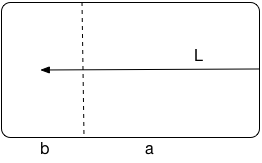
\includegraphics[width=12cm]{q2-2.png}
\caption{将吸收率$I<4$的像素点置0后重建的图像} \label{fig:q2-2}
\end{figure}


\par 通过观察发现发现几乎无影响,说明吸收率$I<4$对应的像素点阵的确是受噪声干扰的无介质区域。

\paragraph*{(2)确定该未知介质在正方形托盘中的位置}~\\

\par 该未知介质左侧距正方形托盘左边缘$28.9044mm$  ,上侧距正方形托盘上边缘$6.2496mm$   ,左右宽度为$44.1378mm$    ,上下长度为 $82.0260mm$ 。
\paragraph*{(3)确定该未知介质的几何形状}~\\
\par 几何形状如图(\ref{fig:q2-2})所示,由一个大椭圆和两个小椭圆组成,其中大椭圆有两个椭圆空洞。整体看来,类似人的头骨。
\newpage
\paragraph*{(4)确定该未知介质的相对吸收率}~\\
\par(1)中得到了新的$256\times 256$的相对吸收率矩阵,因而只需要把10个位置转换成$256\times 256$中的坐标即可读出吸收率。原图$256\times 256$像素中,像素距离为$100/256=0.3906mm$。10个位置以mm为单位的横纵坐标分别除以像素距离取整即得到在原图中的坐标,进而求得要求的相对吸收率。结果如下表(\ref{q2无介质区吸收率置0时求解结果})所示。

\begin{table}[!h]
\centering
\renewcommand\arraystretch{0.6}
\caption{无介质区吸收率置0时求解结果}
\label{q2无介质区吸收率置0时求解结果}
\begin{tabular}{ccc}
\toprule
据左侧边界距离&据下侧边界距离&相对吸收率\\
\midrule
10.0000 &	18.0000 &0.0000\\
34.5000 &	25.0000 &0.9906\\
43.5000 &	33.0000 &0.0000\\
45.0000 &	75.5000 &1.1974\\
48.5000 &	55.5000 &1.0705\\
50.0000 &	75.5000 &1.4772\\
56.0000 &	76.5000 &1.2918\\
65.5000 &	37.0000 &0.0000\\
79.5000 &	18.0000 &0.0000\\
98.5000 &	43.5000 &0.0000\\
\bottomrule 
\end{tabular}
\end{table}


若不将受噪声干扰的无介质区域对应的$I<4$的吸收率置为0,算出的10个位置的相对吸收率结果如下表(\ref{q2无介质区吸收率不置0时求解结果})所示。

\begin{table}[!h]
\centering
\renewcommand\arraystretch{0.6}
\caption{无介质区吸收率不置0时求解结果}
\label{q2无介质区吸收率不置0时求解结果}
\begin{tabular}{ccc}
\toprule
据左侧边界距离&据下侧边界距离&相对吸收率\\
\midrule
10.0000 &	18.0000 &0.0090\\
34.5000 &	25.0000 &0.9906\\
43.5000 &	33.0000 &0.0027\\
45.0000 &	75.5000 &1.1974\\
48.5000 &	55.5000 &1.0705\\
50.0000 &	75.5000 &1.4772\\
56.0000 &	76.5000 &1.2918\\
65.5000 &	37.0000 &0.0046\\
79.5000 &	18.0000 &0.0002\\
98.5000 &	43.5000 &0.0243\\
\bottomrule 
\end{tabular}
\end{table}
\newpage
\subsection{基于小波变换与卷积反投影图像重建模型}
\par 观察附件五中的接收信息矩阵,发现所有点均存在吸收率,因此本文认为附件五的采集数据中必然存在噪声,通过对附件五的接收信息矩阵进行卷积反投影还原,可以得出重构得图像,观察发现重构图像的轮廓不清晰,内部连续性不好,考虑可能存在非线性,非平稳信号,因此采用小波变换\upcite{xiaobo},对图像进行降噪处理。降噪后再进行卷积反投影重构图像,最后求出给定坐标点下的相对吸收率。
\subsubsection{小波变换模型建立}

\par 有用信号通常表现为低频信号或是相对比平稳,而噪声信号通常表现为高频信号。利用小波对含噪的原始信号分解后,含噪部分主要集中在高频小波系数中,并且包含有用信号的小波系数幅值较大,但数目少;而噪声对应的小波系数幅值小,数目较多。
\par 基于上述特点,可以应用门限阈值法对小波系数进行处理,对于较小的小波系数置0,较大的保留,然后对图像重构达到消噪的目的。

\begin{equation}
	\label{q3-eq1}
	W(a,\tau) = \frac{1}{\sqrt{a}}\int_{-\infty}^{+\infty} x(t) \otimes h(\frac{t - \tau}{a}) d \tau
\end{equation}

\par 公式(\ref{q3-eq1})中$W(a,\tau)$为小波变换后的表达式,$x(t)$为原表达式,$h$为选择的小波基,$a$为尺度因子控制小波函数的伸缩,$t$为小波函数的平移量。

\subsubsection{模型求解}
\par 附件5中给出了利用上述CT系统得到的另一个未知介质的接收信息。本文需要利用第一问中得到的标定参数,给出该未知介质的相关信息。另外,需要给出附件4所给的10个位置处的吸收率。通过绘制接收信息的图,可以发现附件5相比附件3而言接收信息轮廓很不清晰,有明显的噪声信号。因而在卷积反投影的基础上,本文加入了小波变换,增加了滤波的功能。
\par 求解算法如下:

\begin{enumerate}
	\item 读取附件5接收信息的数据,存入矩阵$dataTable(512\times180)$中。
	\item 采用db1小波基分解$dataTable$。
	\item 从系数得到近似信号。
	\item 从系数得到细节信号。
	\item 重构信号$dataTable$。
	\item 构造数字滤波器,存入矩阵$hl(1\times 512)$中。
	\item 角度从初始角度(方向为x轴正方向逆时针旋转$61^o$)开始,逐次增加,步长为$1^o$,即循环变量$m$初始值为$1$,逐次增加,步长为$1$,将$dataTable$的第$m$列和$hl$卷积。
	\item 对(7)中确定角度,计算反投影的二维图像,即循环变量$i$、$j$初始值为1,逐次增加,步长为1,将卷积后的结果代入反投影离散求和公式,每次循环进行累加。
	\item (7)、(8)三层循环后计算出$180$次扫描对应二维图像的180次累加,得到还原的二维图像。
	\item 利用问题一中CT系统参数标定将图像进行缩放平移,得到$256\times 256$的原图像。
	\item 对原图像进行阈值处理,将背景置为0,并参照附件三将吸收率归一化为相对吸收率。
	\item 从图像中得到该未知介质在正方形托盘中的位置、几何形状以及附件4中所给的10个位置处的吸收率。
\end{enumerate}

\newpage
\paragraph*{(1)重建图像相关信息}~\\
按照前述方法还原图像如图(\ref{fig:q3-1})所示。
\begin{figure}[h]
\small
\centering
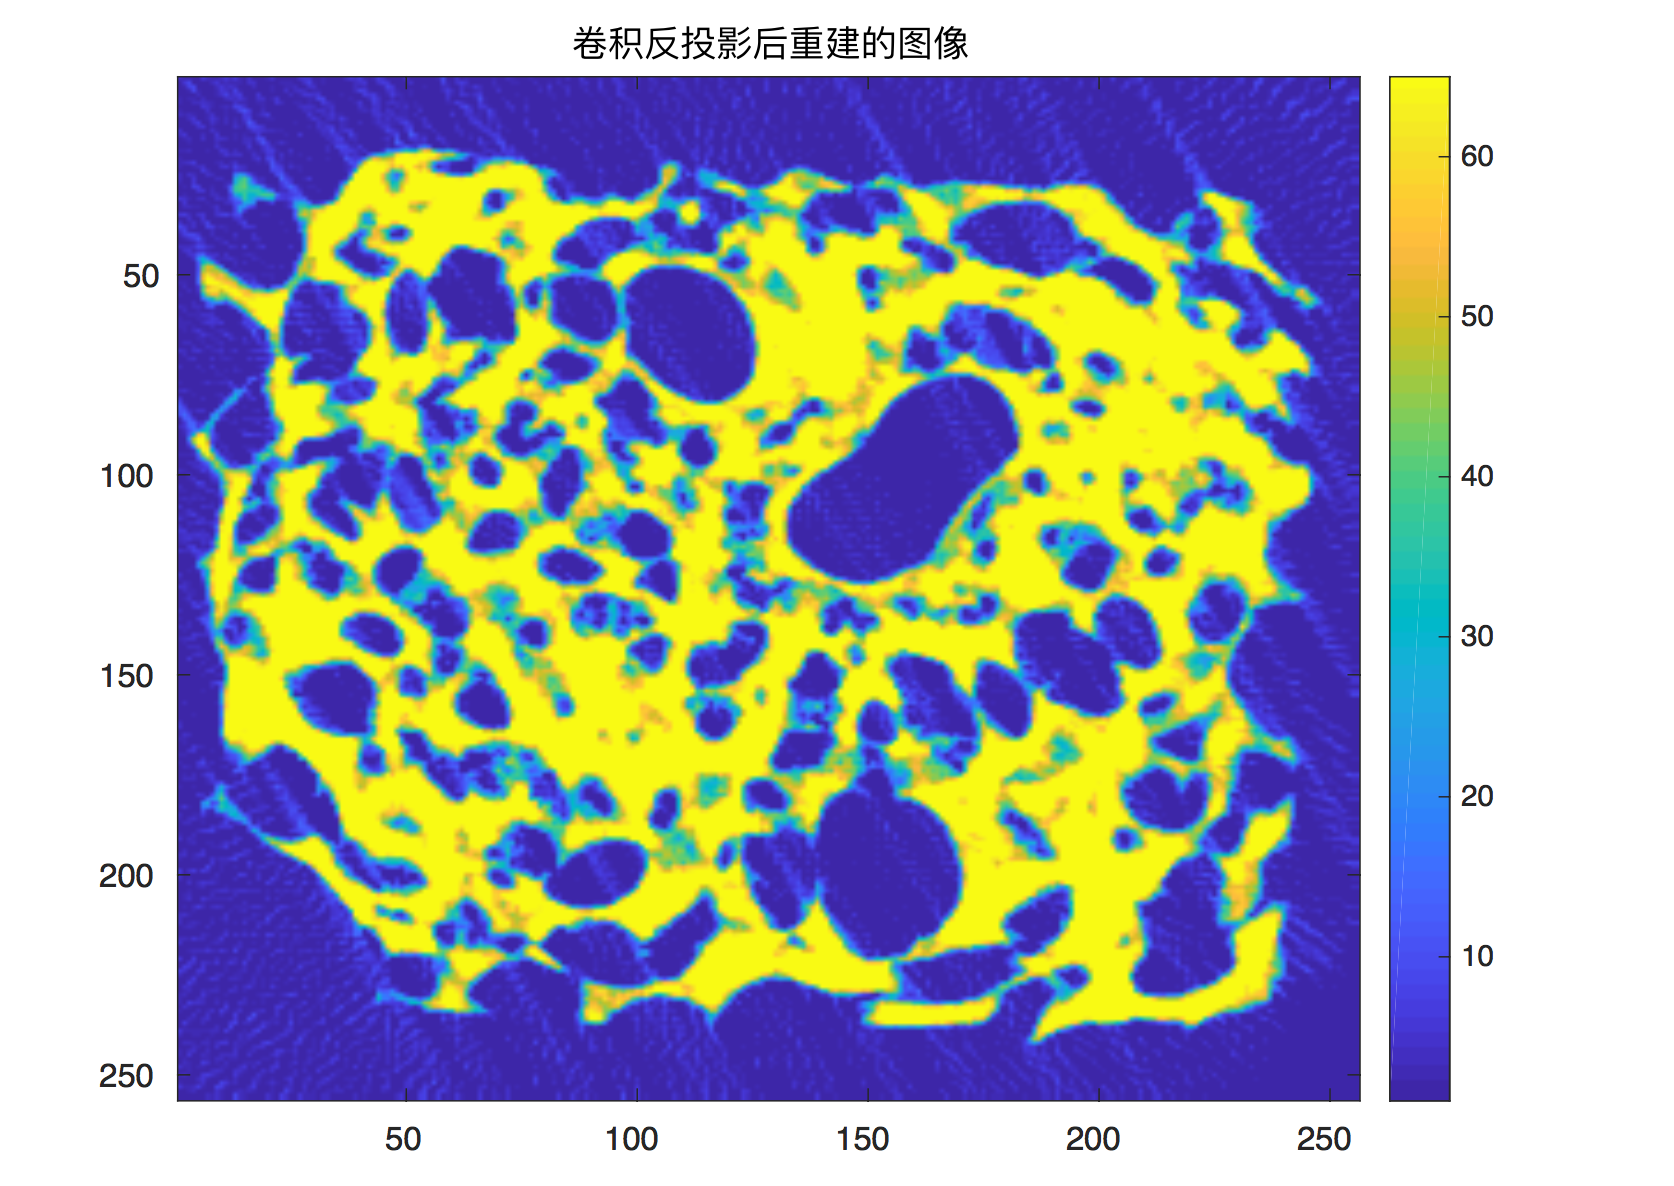
\includegraphics[width=10cm]{q3-1.png}
\caption{卷积反投影后重建的图像} \label{fig:q3-1}
\end{figure}


\par 通过观察可以看到图(\ref{fig:q3-1})中不再是一个形状规则的图形,也不是匀质介质,深浅也表示了不同像素点的吸收率,可能是一块不规整的组织结构。滤波后重建的图像边缘更清晰,每一块块内更连续。

\paragraph*{(2)重建图像的频谱分析}~\\

\par 对表示未滤波重建的原图像和滤波后重建的原图像的矩阵分别转化成单行向量,做快速傅里叶变换进行频谱分析。由图\ref{fig:q3-2}、\ref{fig:q3-3}可以看到,滤波之后的频谱明显更加地平滑,更少有不连续的频率成分,说明滤波的效果很好。
\begin{figure}[!htbp]  
\begin{minipage}[t]{0.5\textwidth}
\centering  
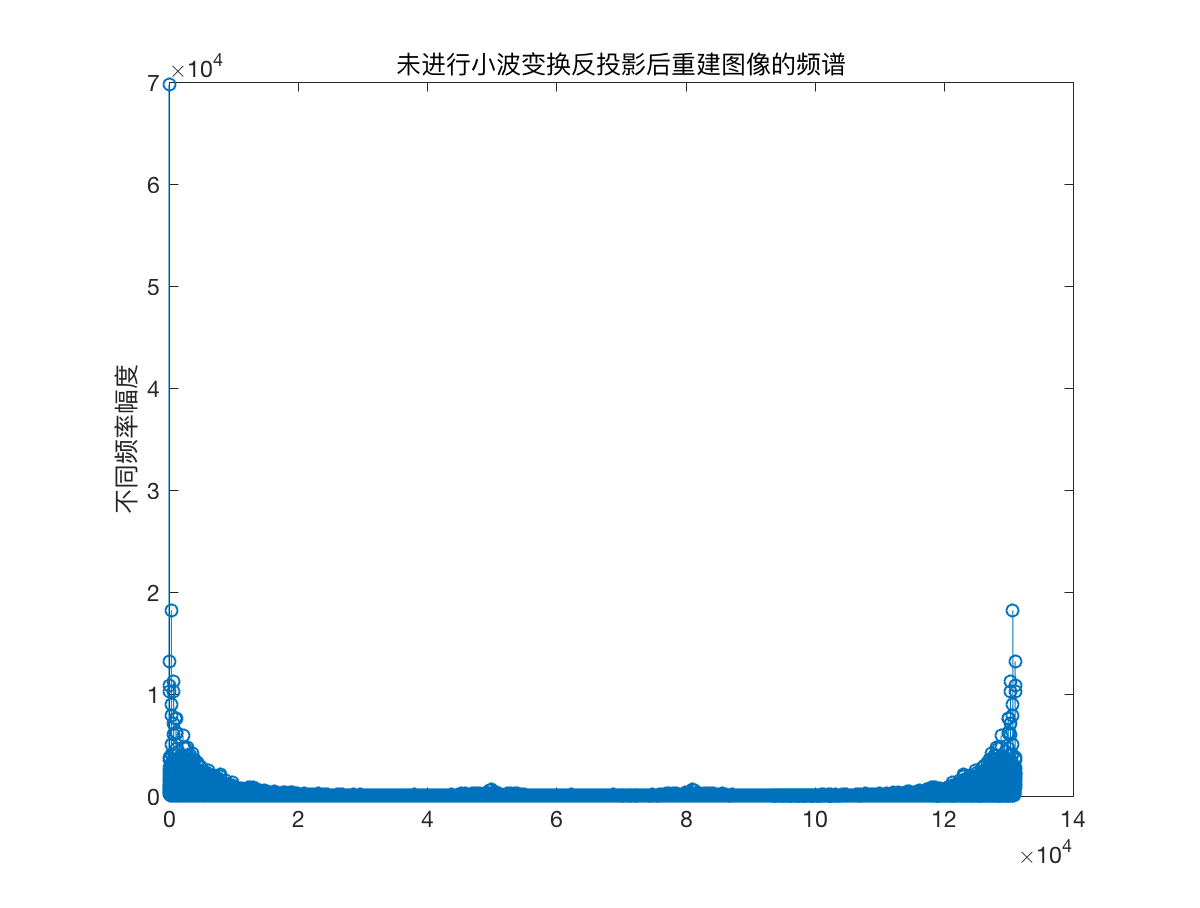
\includegraphics[width=\linewidth]{Q3-1-wei.eps} \\
\caption{未进行小波变换重建图像的频谱} \label{fig:q3-2}
\end{minipage}
\hspace{1ex}
\begin{minipage}[t]{0.5\textwidth}  
\centering  
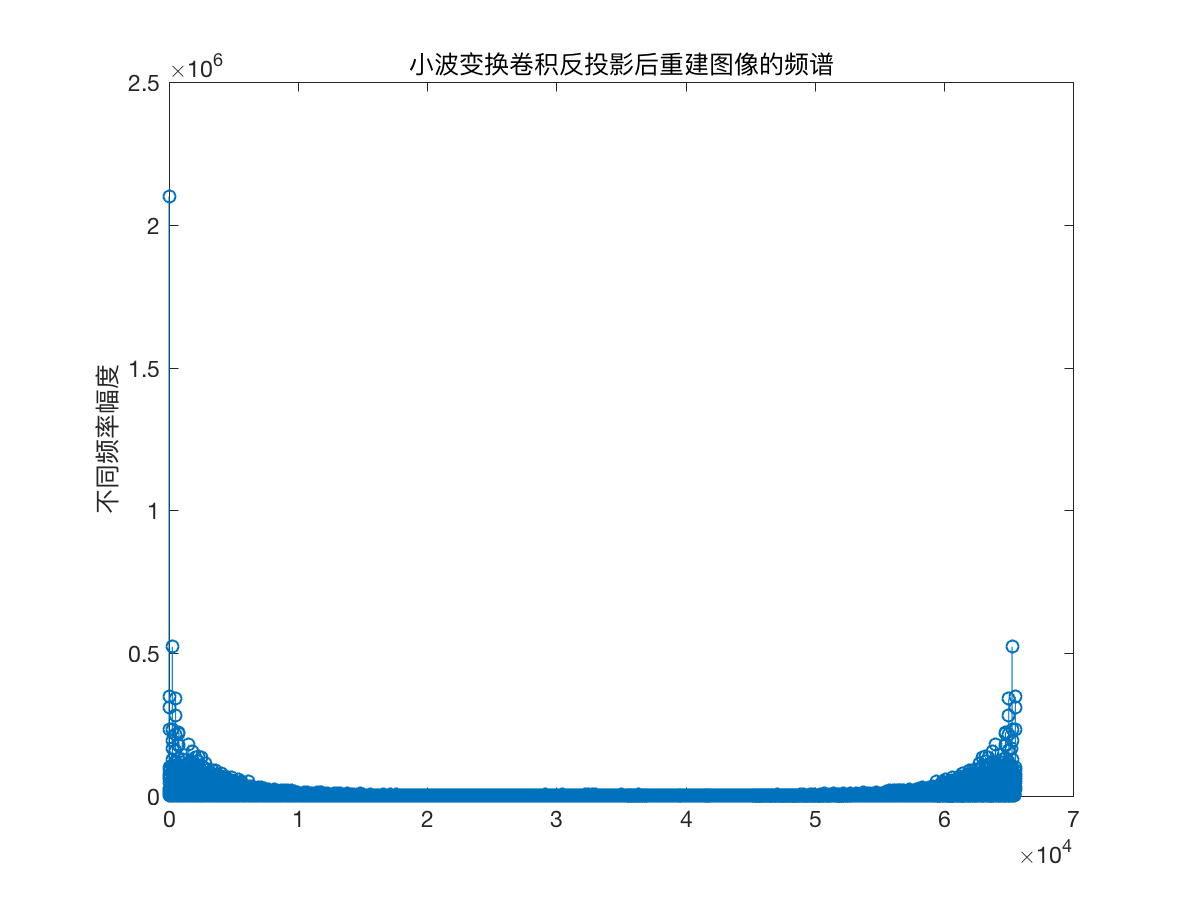
\includegraphics[width=\linewidth]{Q3-2-xiao.eps}\\
\caption{小波变换后重建图像的频谱}  \label{fig:q3-3}
\end{minipage}  
\end{figure} 


\paragraph*{(3)确定该未知介质的相对吸收率}~\\
	
\par 与前一问做法相同,先分析通过附件5重建图像的吸收率,发现由于原图像不匀质也不规则导致吸收率的分布非常离散,此时不再进行阈值处理。直接对吸收率矩阵除以吸收率比例系数得到归一化后的相对吸收率矩阵,因而得到10个点的吸收率如下表(\ref{q3相对吸收率求解结果})所示。
	
\begin{table}[!h]
\centering
\caption{相对吸收率求解结果}
\label{q3相对吸收率求解结果}
\begin{tabular}{ccc}
\toprule
据左侧边界距离&据下侧边界距离&相对吸收率\\
\midrule
10.0000 &	18.0000 &0.0104\\
34.5000 &	25.0000 &2.4336\\
43.5000 &	33.0000 &6.3433\\
45.0000 &	75.5000 &0.0111\\
48.5000 &	55.5000 &0.5005\\
50.0000 &	75.5000 &2.4618\\
56.0000 &	76.5000 &4.7460\\
65.5000 &	37.0000 &0.0898\\
79.5000 &	18.0000 &6.9776\\
98.5000 &	43.5000 &0.1622\\
\bottomrule 
\end{tabular}
\end{table}



\subsection{新标定模型的设计与评价}
\par 在CT仪成像中旋转中心的参数标定对于整个成像过程具有很重要的意义,因此需要选取合适的标定物对旋转中心进行系统的标定,使得对旋转中心的标定经度尽可能的高,且稳定性强。本文将设计出一种新的模板,与原模板相比对旋转中心的标定的经度高,且稳定性强。
\subsubsection{标定模型的设计}
\paragraph*{(1)标定模版外形设计}~\\
\par 对于给定的标定物放置托盘,首先考虑提高托盘的空间利用率,以便于测量标定模版提供更多的信息。其次,通过前述各个小节的分析,本文认为标定物的对称性、极值性(在某一方向上标定物线积分值最大)对于标定模版的标定效果具有显著影响。因此设计具有上述条件的标定模型并进行测试与验证。
\paragraph*{(2)精度与稳定性刻画模型的前提条件}~\\
\par 由在旋转中心固定下对托盘中心的估计,与托盘中心固定下对旋转中心的估计具有相对性。因此在旋转中心确定下对托盘中心位置确定的估计的经度和稳定性,与在托盘中心下旋转中心确定的估计值的经度准确性与否和稳定性等价。
\paragraph*{(3)精度刻画模型的建立}~\\
\par 本文首先给定发射器与接收器的旋转中心,将该旋转中心设置在假想的面积为$512\times 512$像素的旋转区域的中心,如图(\ref{fig:q4-1})所示。然后本文将假想的原尺寸为$256\times 256$像素的托盘(将原$100mm\times 100mm$托盘视作$256\times 256$像素)的中心,随机置于旋转区域中心附近,使得托盘完全置于旋转区域内如图(\ref{fig:q4-2})所示。

\begin{figure}[!htbp]  
\begin{minipage}[t]{0.5\textwidth}
\centering  
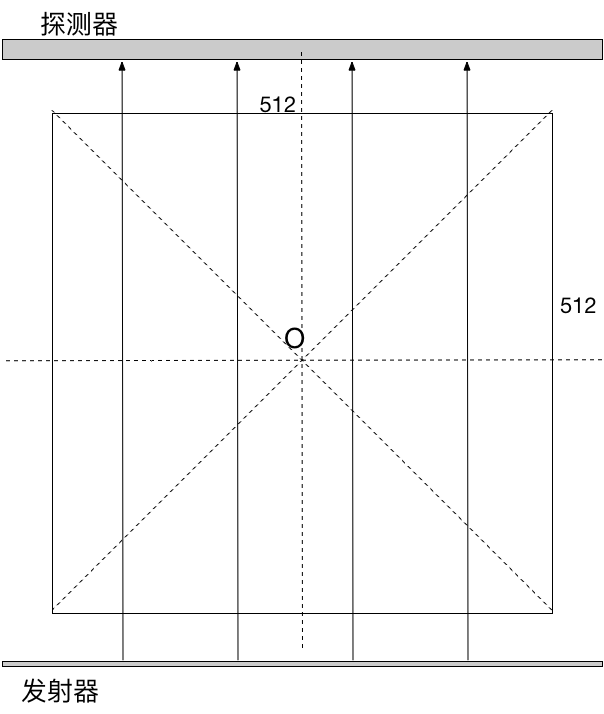
\includegraphics[width=6cm]{q4-1.png} \\
\caption{假想系统示意图} \label{fig:q4-1}
\end{minipage}
\hspace{1ex}
\begin{minipage}[t]{0.5\textwidth}  
\centering  
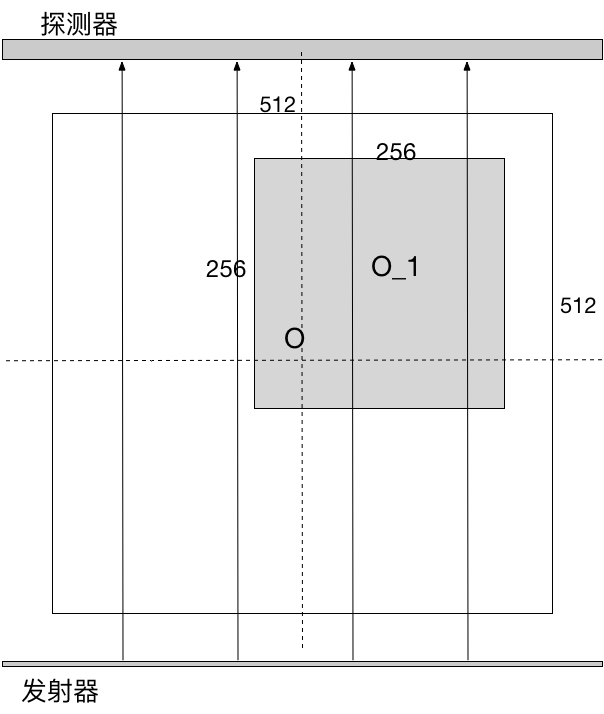
\includegraphics[width=6cm]{q4-2.png}\\
\caption{添加实际托盘后假想系统} \label{fig:q4-2}
\end{minipage}  
\end{figure} 


\par 通过图\ref{fig:q4-1}、\ref{fig:q4-2},本文可以确定出托盘中心与旋转中心的相对位置,(原文中需要确定的是发射器和接收器的旋转中心在托盘中的位置,本文这样设计系统目的是取得给定托盘中心与旋转中心的相对位置)通过某给定的初始位置开始按照每次1°,旋转180次扫描,对接收器每次扫描的接受信息,放置在矩阵中,得到$512\times 180$接收信息矩阵。
\par 将该接收信息矩阵进行色阶图处理,通过与第一问相同的方法,通过色阶图中的特殊位置确定出新的托盘中心的位置。该托盘位置为本文通过色阶图的到托盘中心的估计位置,同时也就得到旋转中心在托盘中的相对估计位置。
\par 通过改变标定模板,不断计算得出估计出托盘中心的位置与原来托盘中心确定位置间的距离。如果新设计模板的距离比原模板的距离小,可以得出新设计出的标定模板的经度大于原设计模板的精度。

\par 因而本文对精度的衡量提出两个指标。一是托盘中心真实值$O_0$和计算值$O_0’$的差$\varepsilon$,(公式(\ref{q4-eq-1})所示)二是通过标定之后重建图像与原图像的重合度。(公式(\ref{q4-eq-2})所示)对于托盘中心真实值和计算值的差,实则是对求解旋转中心真实值和标定值之差问题的转化。标定模板均为匀质介质,因而将重建图像和原图像通过阈值分析二值化后,原图像吸收率相同的像素点个数为$Q'$,重建图像像素点个数为$Q$,重合度$S$即为$Q’$与$Q$的比值。
\begin{equation}
	\label{q4-eq-1}
	\varepsilon = \mid O_0' - O_0 \mid \times 100\%
\end{equation}

\begin{equation}
	\label{q4-eq-2}
	S = \frac{Q'}{Q} \times 100\%
\end{equation}

\paragraph*{(4)稳定性刻画模型的建立}~\\

\par 由于在实际的操作过程中外界的噪声会对系统产生影响,本文通过添加不同功率的噪声,按照上述方法分别计算出不同功率噪声下的旋转中心,在本文改变噪声功率的过程中,如果新建立的模板在不同功率噪声影响下建立的出的旋转中心与不加噪声时的托盘中心的平均偏差比原模板小,则可以说明该新模板的稳定性更高。
\par 对稳定性的讨论本文同时考虑,对于开始检测的初始角度的设置改变时系统标定参数的变动。例如:若改变初始角度时标定得到的旋转中心与实际旋转中心的距离的变化。因而本文对稳定性的衡量沿用托盘中心真实值$O_0$和计算值$O_0’$的差$\varepsilon$(如公式(\ref{q4-eq-2})所示)。

\subsubsection{标定模型的评价}
本文给出一种较优的标定模版设计如图(\ref{fig:q4-3})所示,同时检验了其他几种不同的设计方案,但均相较于原有标定模版精度较低,以两种设计为例(如图\ref{fig:q4-3-1}、\ref{fig:q4-3-1}所示)。

\begin{figure}[!htbp]  
\begin{minipage}[t]{0.3\textwidth}
\centering  
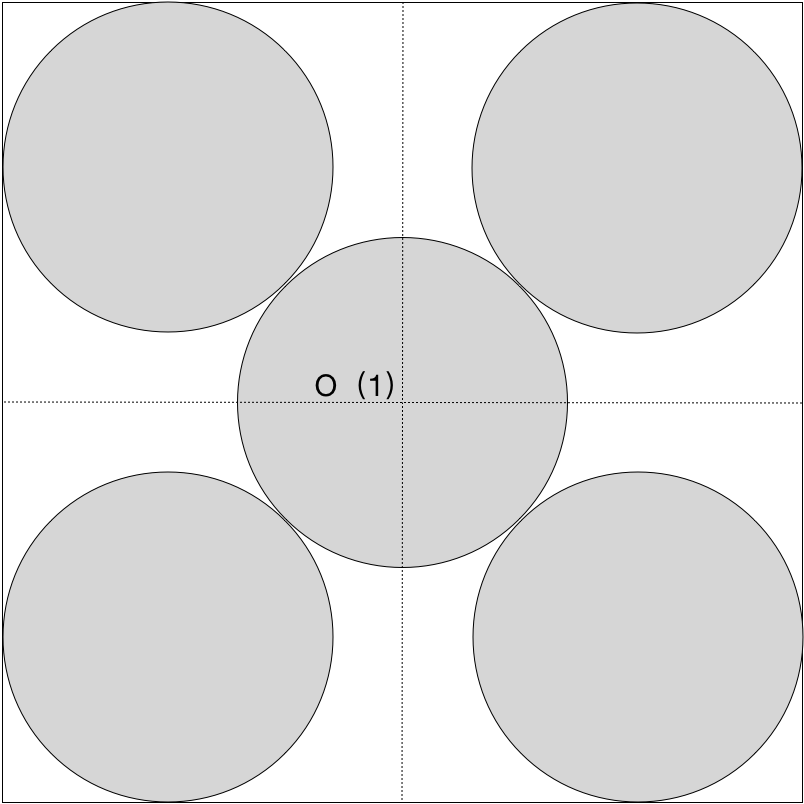
\includegraphics[width=\linewidth]{q4-3.png}
\caption{较优设计方案} \label{fig:q4-3}
\end{minipage}
\hspace{1ex}
\begin{minipage}[t]{0.3\textwidth}
\centering  
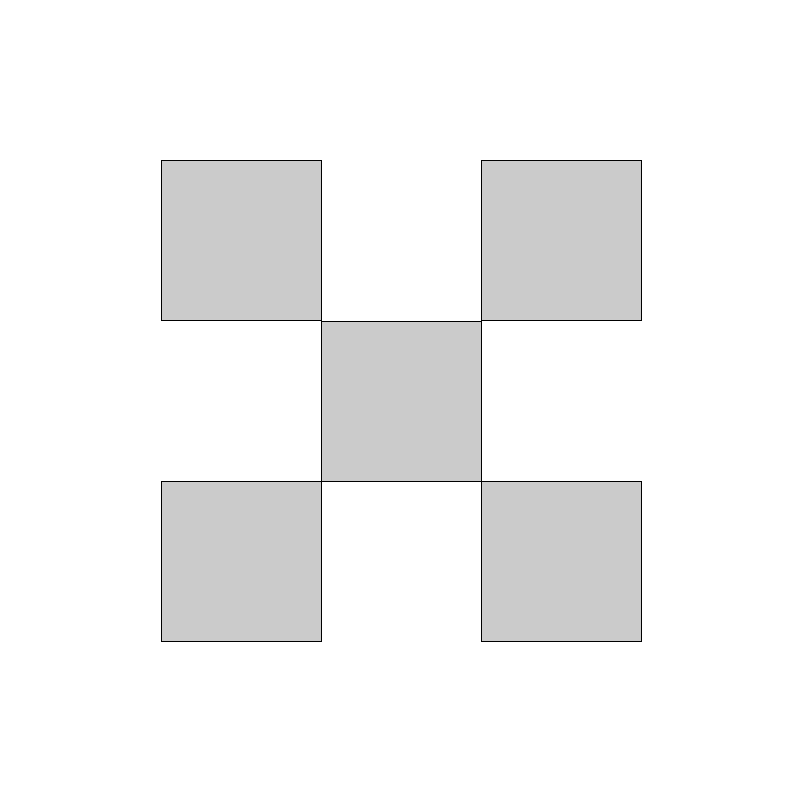
\includegraphics[width=\linewidth]{q4-plan3.png} \\
\caption{其他方案(1)} \label{fig:q4-3-1}
\end{minipage}
\hspace{1ex}
\begin{minipage}[t]{0.3\textwidth}  
\centering  
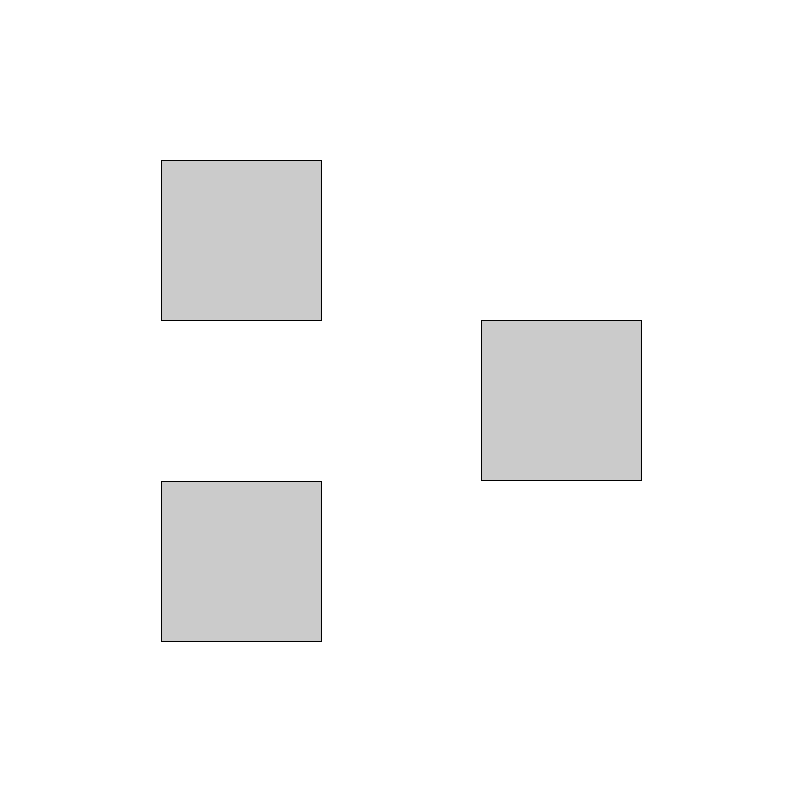
\includegraphics[width=\linewidth]{q4-plan4.png}\\
\caption{其他方案(2)} \label{fig:q4-3-1}
\end{minipage}  
\end{figure} 

\newpage
\paragraph*{(1)参数标定的精度评价}~\\
对本文设计的标定模型,建立如下图(\ref{fig:q4-4})所示的平面直角坐标系:

\begin{figure}[!htbp]  
\begin{minipage}[t]{0.5\textwidth}
\centering  
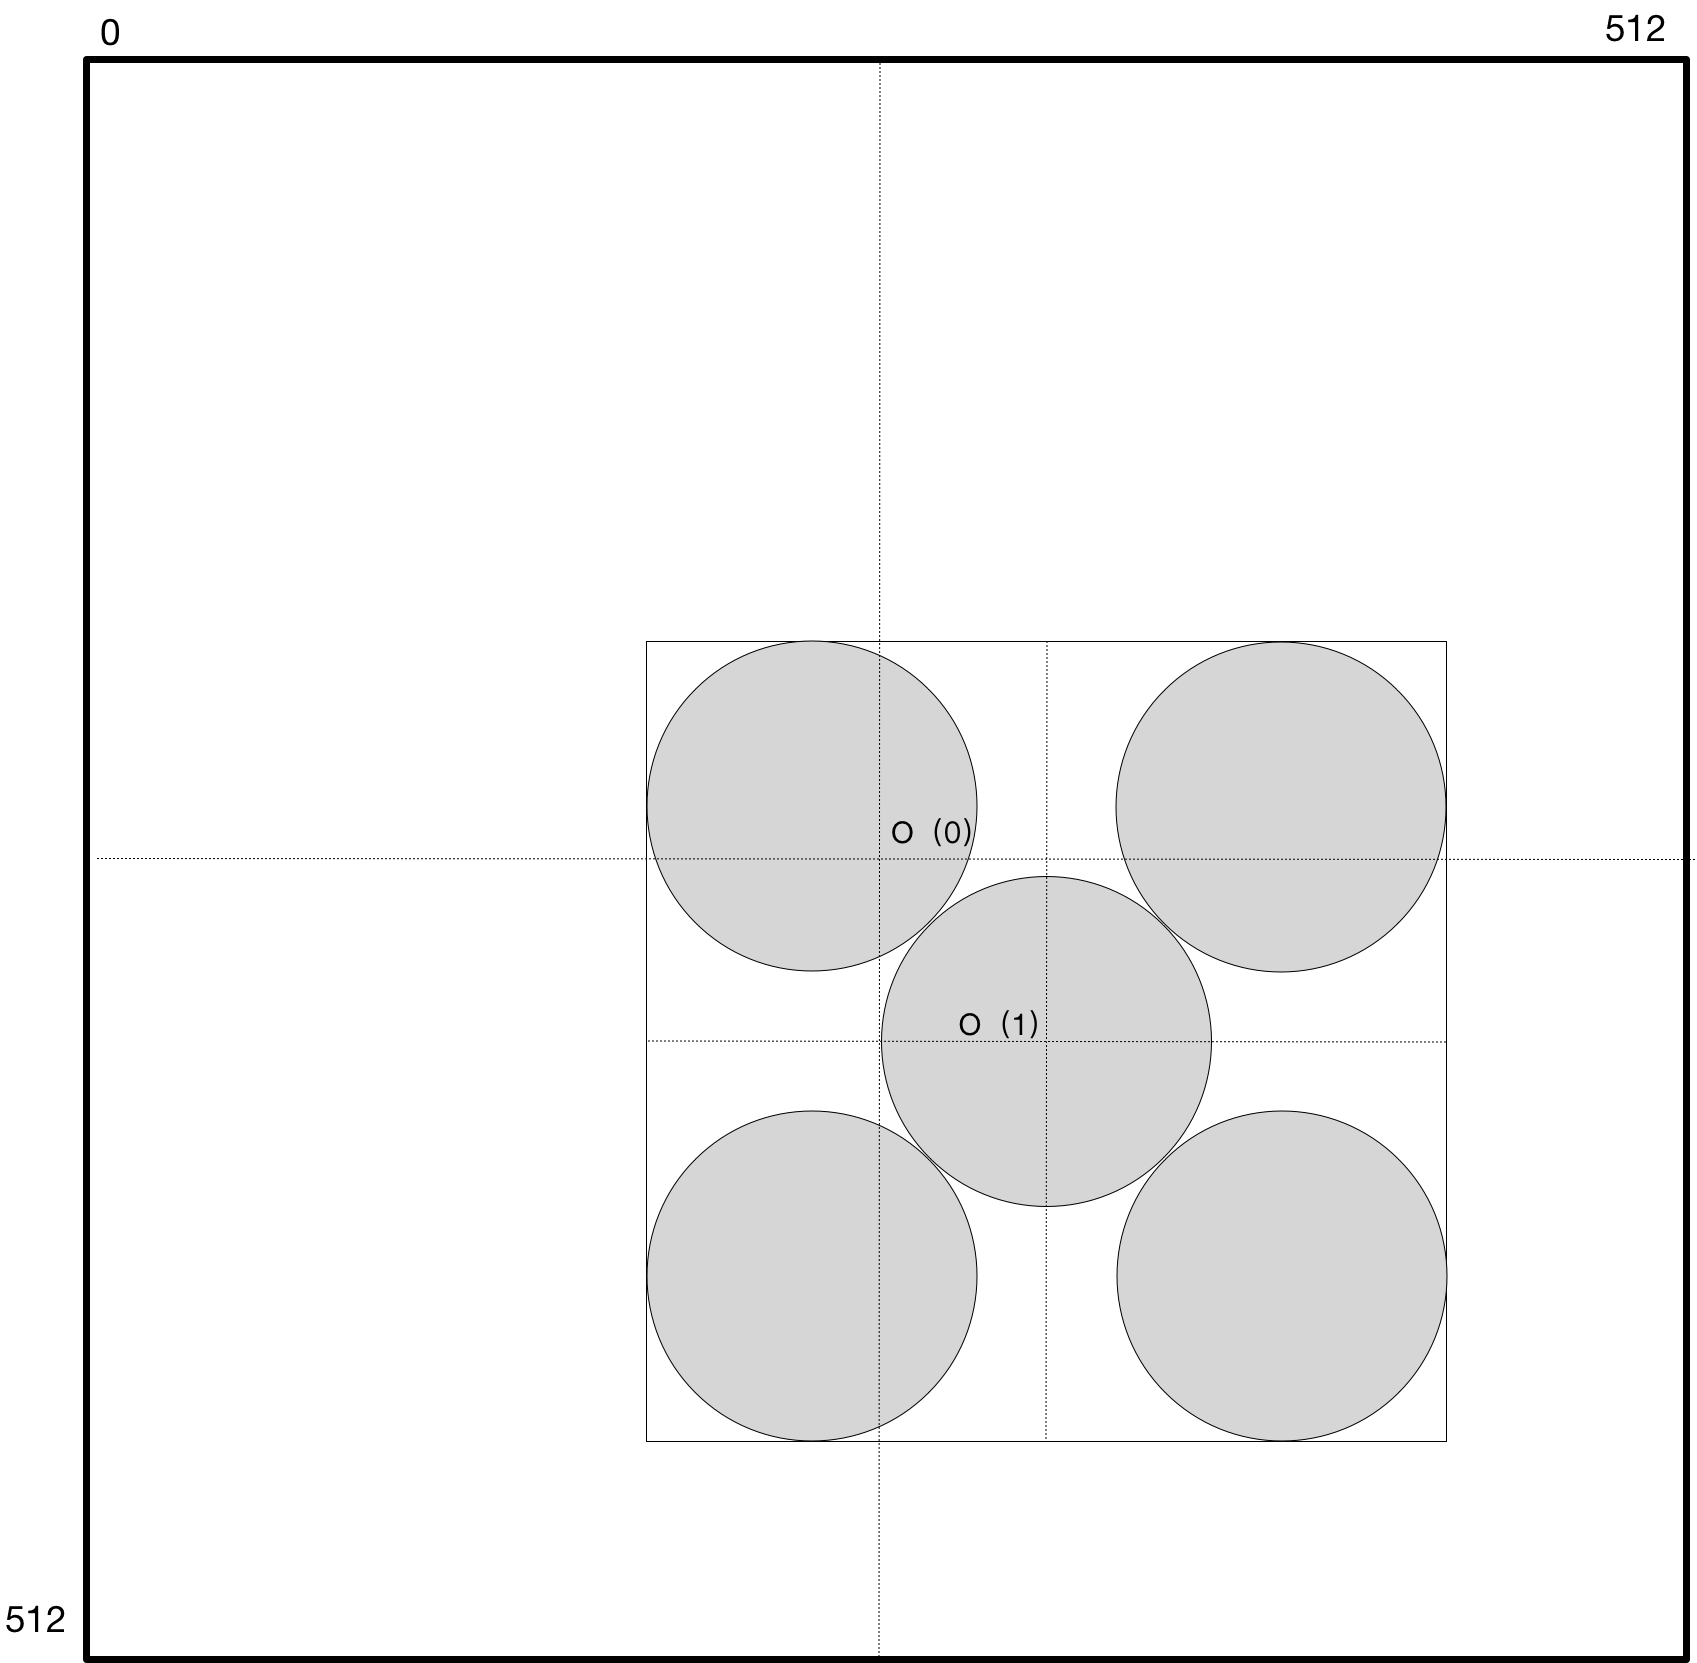
\includegraphics[width=\linewidth]{q4-4.png} \\
\caption{坐标系建立} \label{fig:q4-4}
\end{minipage}
\hspace{1ex}
\begin{minipage}[t]{0.5\textwidth}  
\centering  
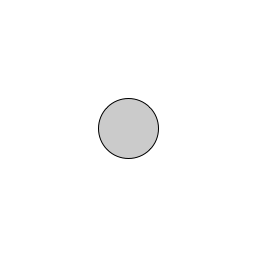
\includegraphics[width=\linewidth]{q4-base.png}\\
\caption{重合度测量基准图形} \label{fig:q4-base}
\end{minipage}  
\end{figure} 


从图中(该图为示意图)可以看出,正方形托盘的中心在位置,整个旋转中心的位置为,对这两个中心本文预先给定。

对于中心距离差值的计算假设本文给定$O_1$坐标为(229,279),$O_0$坐标为(256,256),通过问题一中的的初始位置(与x轴正方向顺时针夹角为61°)开始按照每次1°,逆时针旋转180次扫描,对接收器每次扫描的接受信息,放置在矩阵中,得到$512\times 180$接收信息矩阵,将接受信息的矩阵转换为色阶图,如下图(\ref{fig:q4-sejie2})所示:

\begin{figure}[h]
\small
\centering
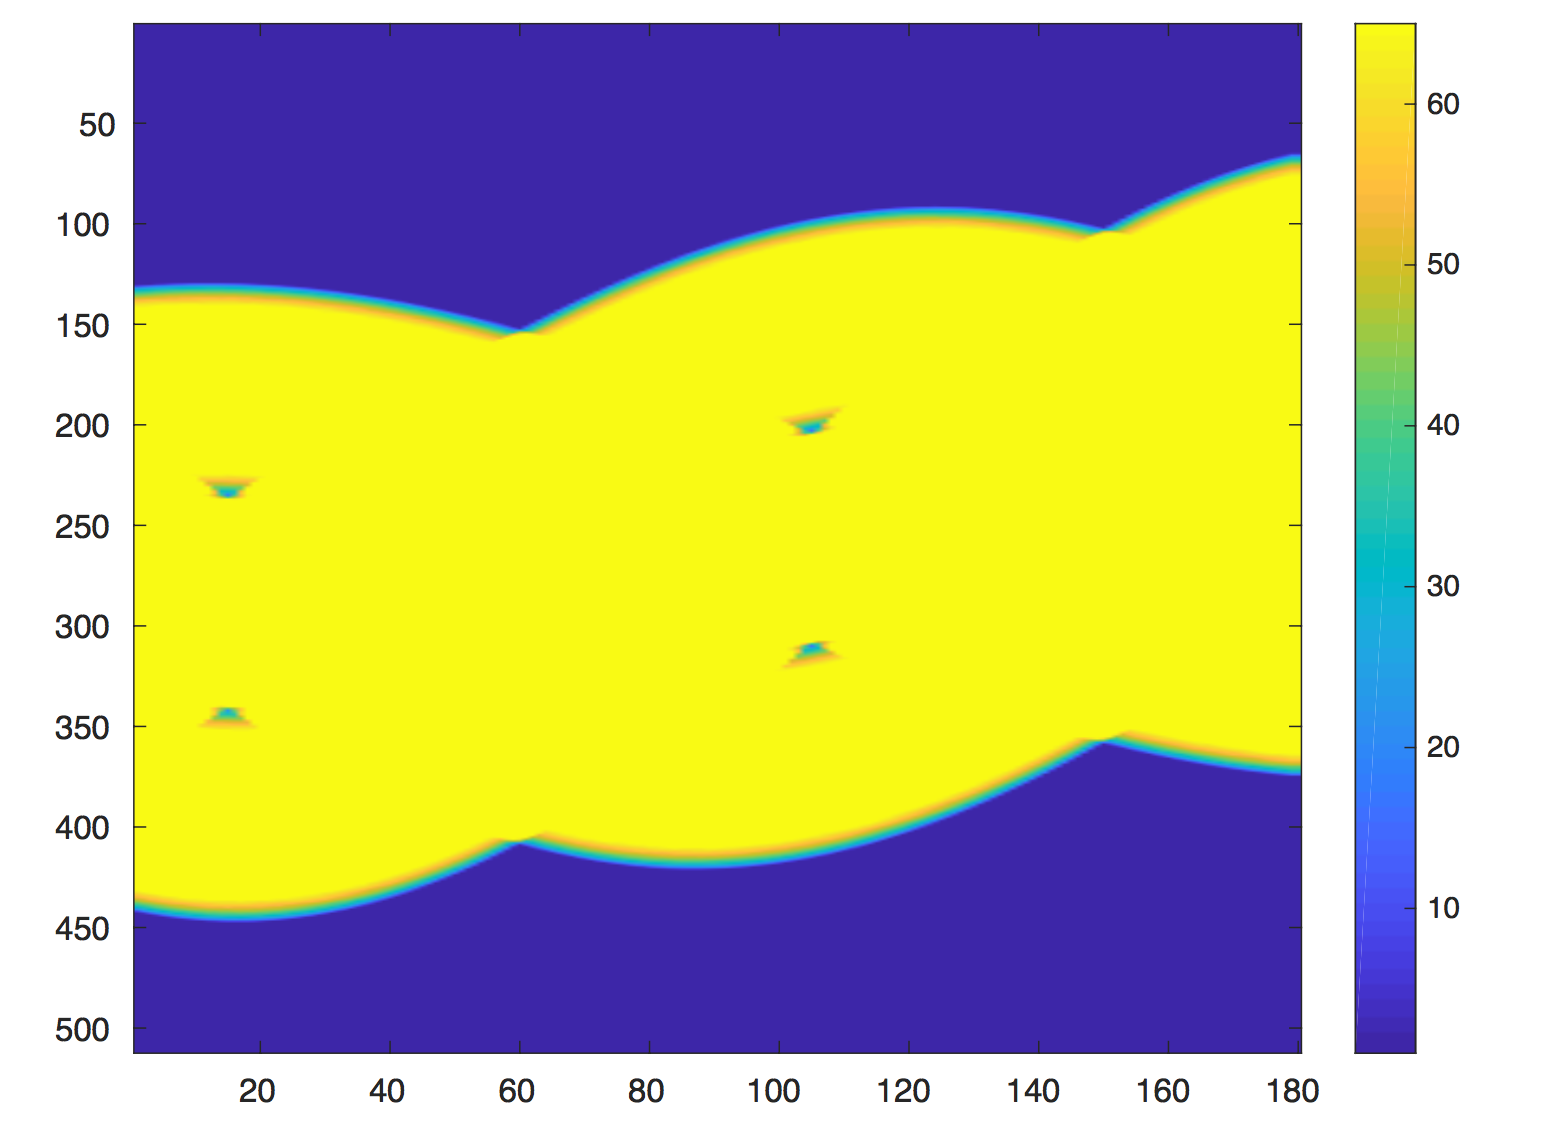
\includegraphics[width=9cm]{q4-sejie2.png}
\caption{接收信息矩阵色阶图} \label{fig:q4-sejie2}
\end{figure}

通过上述色阶图(\ref{fig:q4-sejie2}),本文得出确定出托盘中心位置的两个关键列分别为第61列和151列,可以得出通过色阶图确定出的$O_0'$坐标为(231,283)与$O_0$(229,279)的距离经计算为$\varepsilon_{new} = 4.4721$。重建图像重合

将原有标定模版所在的小托盘放置在前述方案中小托盘位置,其余计算方法参见问题一、二中的计算模型。可以得出通过色阶图确定出$O_0'$的坐标为(234,283)与$O_0$(229,279)的距离经计算为$\varepsilon_{old} = 6.4031$。

通过两种模板下方形托盘旋转中心的理论位置与实际位置的距离$\varepsilon_{new}<\varepsilon_{old}$,

设置重合度计算标准模版如图(\ref{fig:q4-base})所示,分别计算出两种方案的重合度,新标定模版的重合度$S_{new} = 0.9919$,旧标定模版的重合度$S_{old} = 0.9899$。

综上所述,结合重合度和中心间距离差两个指标,本文设计模版的精度均要好于原模板。

\paragraph*{(2)参数标定的稳定性评价}~\\
\par 本文通过添加不同功率的噪声,按照前述方法分别计算出不同功率噪声下的托盘中心,在本文改变噪声功率的过程中,如果某种新模板在不同功率噪声影响下建立的出的托盘中心与不加噪声时的托盘中心的平均偏差比原模板小,则可以说明该新模板的稳定性更高。分别添加50dB,100 dB ,150dB,200dB,1000dB的高斯白噪声,可以得出对两种模板下,托盘中心的测定结果,如下表(\ref{不同噪声水平下模版对旋转中心标定的结果})所示:

\begin{table}[!h]
\centering
\caption{不同噪声水平下模版对旋转中心标定的结果}
\label{不同噪声水平下模版对旋转中心标定的结果}
\begin{tabular}{ccc}
\toprule
噪声大小(db)&原标定模版&新标定模版\\
\midrule
50   & (242,291) & (231,283) \\
100  & (242,291) & (231,283) \\
150  & (242,291) & (231,283) \\
200  & (242,291) & (231,283) \\
1000 & (243,291) & (233,283) \\
\bottomrule 
\end{tabular}
\end{table}

\par 通过上表求解发现加不同功率高斯白噪声下,原方案计算的托盘中心坐标和实际托盘中心坐标一致。本文提的新方案计算的托盘中心坐标和实际托盘中心坐标也一致,说明新方案的抗噪声性能很好。分析原因是因为标定模板具有对称性,随机噪声对其影响不大。

\par 本文探求初始参数的设置值对两种标定模板在旋转中心确定后,通过卷积反投影图像重建重合度的影响。因此将开始检测的初始角度的设置值分别为61°62°71°81°90°(其中这些角度均为与x正半轴顺时针夹角),测量各初始角度下对基准图像还原的重合度如下表(\ref{相对吸收率求解结果})所示。

\begin{table}[!h]
\centering
\caption{相对吸收率求解结果}
\label{相对吸收率求解结果}
\begin{tabular}{ccc}
\toprule
初始角度($^o$)&原标定模版&新标定模版\\
\midrule
61 & 0.9899 &0.9919\\
62 &0.9899 &0.9919\\
71 &0.9899 &0.9921\\
81 &0.9899 &0.9923\\
90 &0.9899 &0.9924\\
\bottomrule 
\end{tabular}
\end{table}


\par 通过对初值的变动,最终本文得出的我们设计出的新的标定模板还原图像的重合度比原模板还原图像的重合度高,因此本文新设计出的模板的稳定性较强。

\section{模型评价与改进}
\subsection{模型优点}
\begin{enumerate}
	\item 在参数标定的过程中,对每次的旋转角度给出估计值,并运用卷积反投影对估计出的值进行检验
	\item 卷积反投影可消除单纯的反投影产生的边缘失锐效应,保证重建图像边缘清晰和内部分布均匀。
	\item 运用小波变换使得图像轮廓清晰,内部分布均匀。
\end{enumerate}
\subsection{模型缺点}
\begin{enumerate}
	\item 没有充分考虑180个方向非等间隔扫描的情况。
	\item 问题四中,本文对影响参数标定的因素考虑不够充分,例如标定模版对称性等。
\end{enumerate}

\subsection{模型改进}
对于第四问设计的新模板,我们可以对探究影响标定参数经度的影响因素,如标定模板占方形托盘的面积比例,标定模板的对称性,标定物的形状对旋转中心参数标定的影响。


\begin{thebibliography}{9}
 \bibitem{fuliye} 杨文, 何楚. 二维傅立叶变换的教学实践[J]. 电气电子教学学报, 2014, 36(2):30-32.
 \bibitem{fuliyeqiepian} 于飞. 基于断层切片的血管造影三维重建[D]. 西安电子科技大学, 2007.
 \bibitem{xiaobo} 潘泉, 孟晋丽, 张磊,等. 小波滤波方法及应用[J]. 电子与信息学报, 2007, 29(1):236-242.
\end{thebibliography}

\section{附件清单}
\begin{enumerate}
	\item 通过附件二重建的吸收率矩阵中不同吸收率范围对应像素点的个数-数据表
	\item 通过附件三重建的吸收率矩阵中不同吸收率范围对应像素点的个数-数据表
	\item 通过附件五重建的吸收率矩阵中不同吸收率范围对应像素点的个数-数据表
	\item 基于数据表格模拟图像扫描matlab程序
	\item 基于设计图的模拟图像扫描matlab程序
	\item 通过基准物的扫描结果数据还原图像matlab程序
\end{enumerate}
\newpage
\section{附件}
\subsection{关键数据}

\textbf{通过附件二重建的吸收率矩阵中不同吸收率范围对应像素点的个数}

\begin{figure}[h]
\small
\centering
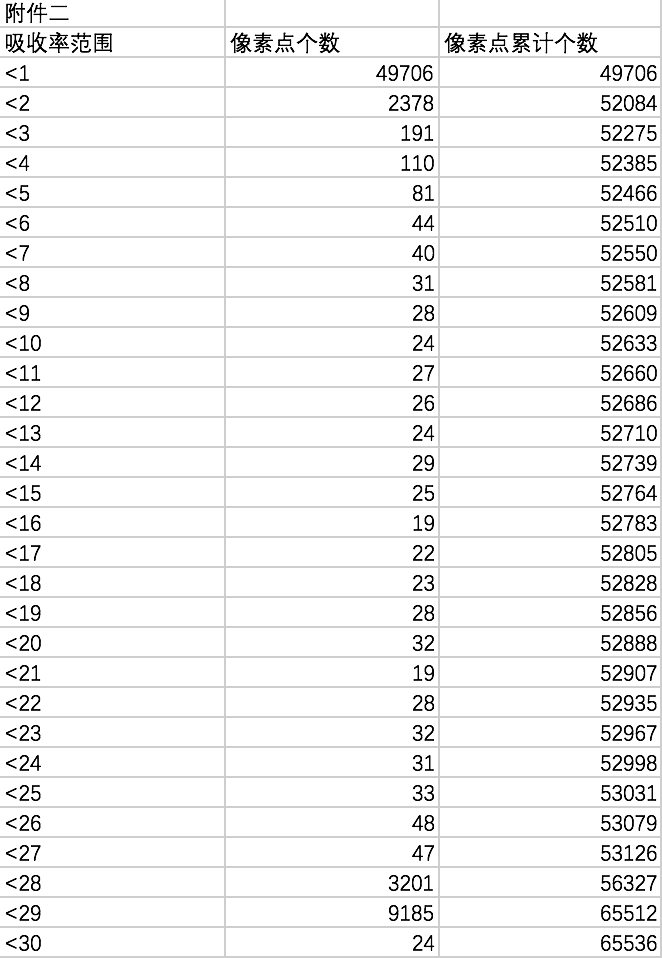
\includegraphics[width=12cm]{q2-fu2-1.png}
\caption{} \label{fig:q2-fu2-1}
\end{figure}
\newpage
\textbf{通过附件三重建的吸收率矩阵中不同吸收率范围对应像素点的个数}

\begin{figure}[h]
\small
\centering
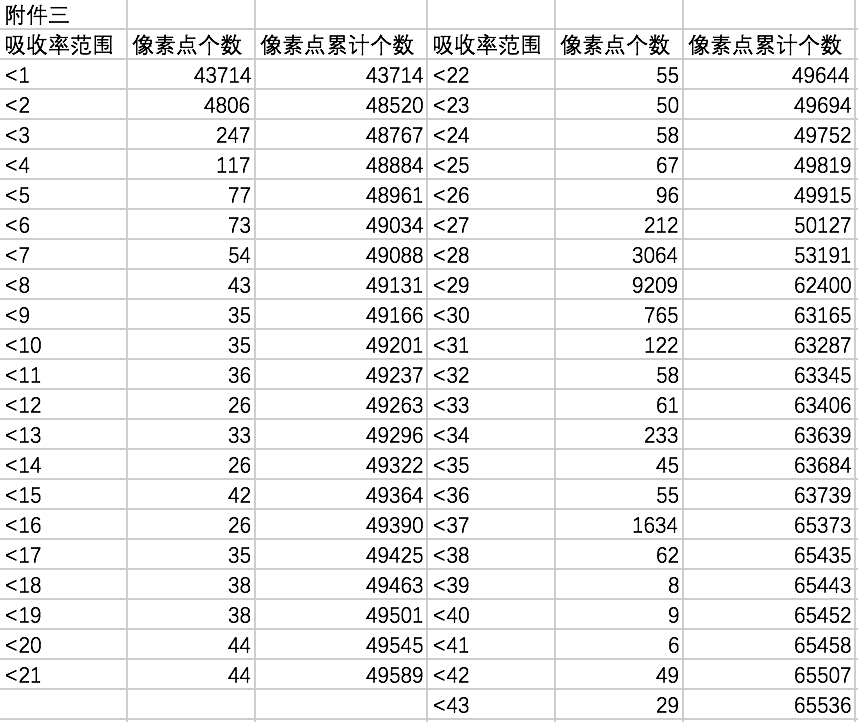
\includegraphics[width=\textwidth]{q2-fu3-1.png}
\caption{} \label{fig:q2-fu3-1}
\end{figure}
\newpage
\textbf{通过附件五重建的吸收率矩阵中不同吸收率范围对应像素点的个数}

\begin{figure}[h]
\small
\centering
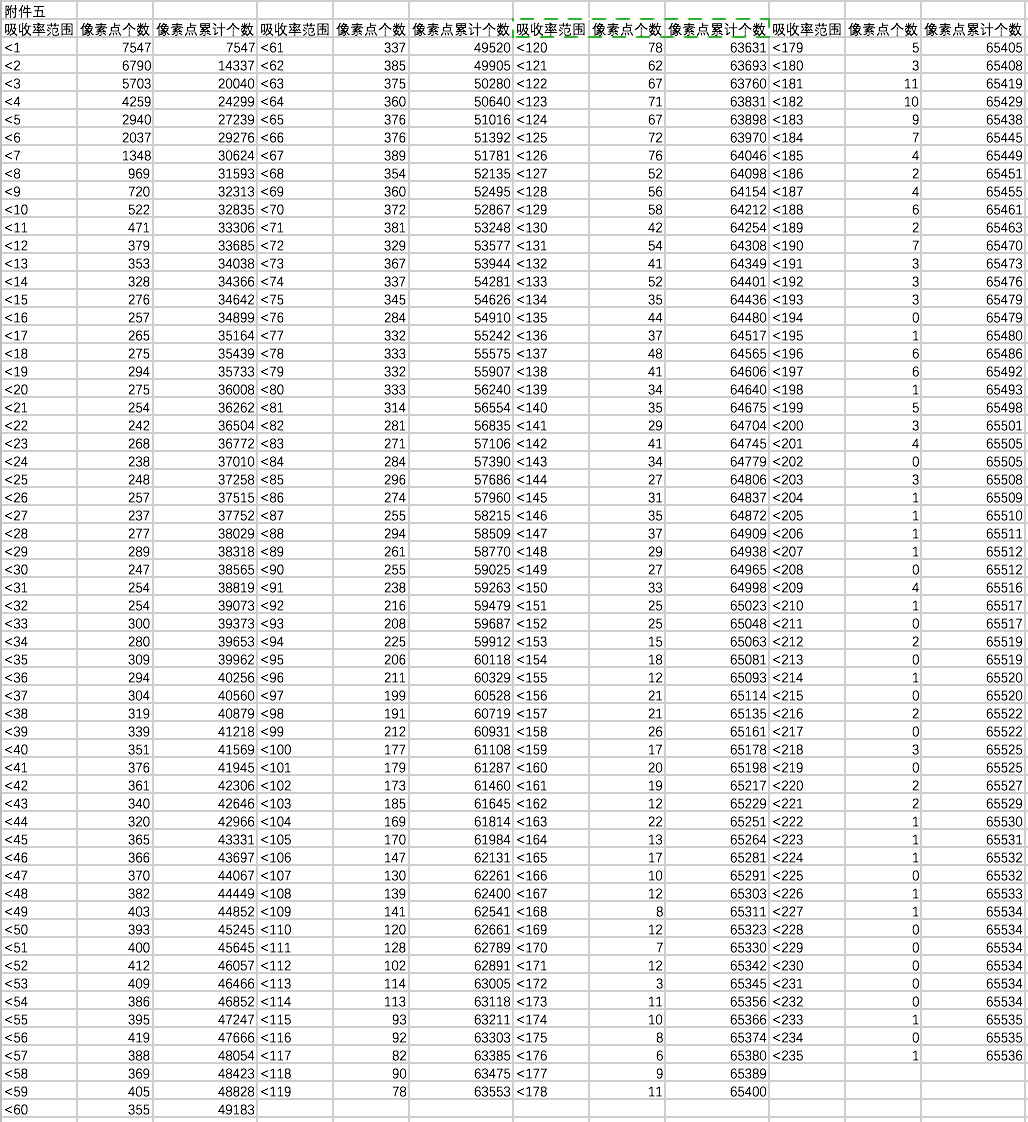
\includegraphics[width=\textwidth]{q3-fu5-1.png}
\caption{} \label{fig:q3-fu5-1}
\end{figure}
\newpage
\subsection{程序源代码}
\textbf{基于数据表格模拟图像扫描}
% 代码插入,请将代码文件放入code文件夹,支持语言的语法高亮。支持语言:C,C++,Java,Matlab,Mathematica,python,R,可在cls文件中自行添加。
\lstinputlisting[language=C++]{./code/q4_plan0_pic.m}

\textbf{基于设计图的模拟图像扫描}
\lstinputlisting[language=C++]{./code/q4_plan1_pic.m}

\textbf{通过基准物的扫描结果数据还原图像}
\lstinputlisting[language=C++]{./code/q4_re.m}

\end{document} 